\documentclass[12pt]{article}
\usepackage[utf8]{inputenc}
\usepackage[margin=1.5in]{geometry}
\usepackage{graphicx}
\usepackage{amsmath}
\usepackage{amssymb}
\usepackage{titlesec}
\usepackage{listings}
\usepackage{xcolor}
\usepackage[hidelinks]{hyperref}
\hypersetup{
    citecolor=black,
    filecolor=black,
    linkcolor=black,
    urlcolor=black
}

\definecolor{codegreen}{rgb}{0,0.6,0}
\definecolor{codegray}{rgb}{0.5,0.5,0.5}
\definecolor{codepurple}{rgb}{0.58,0,0.82}
\definecolor{backcolour}{rgb}{0.95,0.95,0.92}

\lstdefinestyle{codestyle}{
    backgroundcolor=\color{backcolour},
    commentstyle=\color{codegreen},
    keywordstyle=\color{magenta},
    numberstyle=\tiny\color{codegray},
    stringstyle=\color{codepurple},
    basicstyle=\ttfamily\footnotesize,
    breakatwhitespace=false,
    breaklines=true,
    captionpos=b,
    keepspaces=true,
    numbers=left,
    numbersep=5pt,
    showspaces=false,
    showstringspaces=false,
    showtabs=false,                  
    tabsize=2
}

\lstset{style=codestyle}
\setcounter{secnumdepth}{4}

\title{Reti di Telecomunicazioni - Domande Frequenti}
\author{Autore: Giovanni Orciuolo - Matricola 574268}
\date{Docente del corso: Prof. Gennaro Boggia}

\renewcommand*\contentsname{Sommario}

\begin{document}
\graphicspath{ {./images/} }

\begin{titlepage}
    \begin{center}
        \vspace*{1cm}
            
        \Huge
        \textbf{Reti di Telecomunicazioni}
            
        \vspace{0.5cm}
        \LARGE
        Domande Frequenti
            
        \vspace{1.5cm}
            
        \textbf{Autore: Giovanni Orciuolo}
            
        \vfill
            
        Docente del corso: Prof. Gennaro Boggia
            
        \vspace{0.8cm}
            
        
\includegraphics[width=0.4\textwidth]{logo_poliba}
        
        \vspace{0.8cm}
        \Large
        Politecnico di Bari\\
        Corso di Laurea in Ingegneria Informatica\\
        1 Luglio 2021
        
        \vspace{1cm}
        Made with \LaTeX\\
        MS Word can kiss my ass
    \end{center}
\end{titlepage}

\newpage
\tableofcontents
\newpage

\section{Domande sul layer TCP/IP}

\subsection{Caratteristiche UDP e formato datagramma}

Il protocollo UDP (User Datagram Protocol) è un protocollo \textbf{connection-less}, pertanto fornisce un servizio inaffidabile e non si assicura in alcun modo che i pacchetti arrivino effettivamente al destinatario. Dunque la sua unica funzione è il \textbf{multiplexing}. Una PDU in UDP è detta "\textbf{datagram}".
Un datagram è composto da \textbf{header} e \textbf{payload}. Nell'header sono presenti la \textbf{source port}, la \textbf{destination port}, la \textbf{length} (lunghezza del datagram in byte) e il \textbf{checksum}. Il campo checksum consiste in un valore calcolato sommando 16 bit a 16 bit il contenuto del datagram e dello \textbf{pseudoheader} (che contiene anche gli indirizzi IP mittente e destinatario). Il risultato viene complementato a 1. In ricezione, il processo viene ripetuto e si controlla che il risultato siano tutti 1. Se così non fosse, c'è stato un errore, e il datagram viene scartato. In questo contesto non ci sono meccanismi di ritrasmissione di alcun tipo.

\subsection{Three-Way Handshake}

Il Three-Way Handshake è il meccanismo mediante il quale viene \textbf{inizializzata una connessione} in TCP.
Per prima cosa, il \textbf{client invia al server} un pacchetto contenente la flag \textbf{SYN=1} (indica il desiderio di inizializzare una connessione) e il \textbf{Sequence Number} a un valore \textbf{x}. Questo valore è scelto casualmente dal client e sarà la base di numerazione dei suoi byte trasmessi per quella connessione. Il \textbf{server risponde} con flags \textbf{SYN=1}, \textbf{ACK=1}, \textbf{Sequence Number} a \textbf{y}, dove y è il numero casuale scelto dal server e sarà la sua base di numerazione per i byte trasmessi dalla sua parte per la connessione) e \textbf{ACK Number = x+1}.
Il \textbf{client risponde} nuovamente con \textbf{ACK=1}, \textbf{Sequence Number = x+1} e \textbf{ACK Number} pari a \textbf{y+1}. Senza attendere riscontro dal server, manda un nuovo pacchetto, stavolta però con payload corrispondente ai primi byte da trasmettere. In alcune implementazioni di TCP, questi ultimi 2 passaggi sono uniti. Di seguito lo schema del Three-Way Handshake realizzato dal docente:

\begin{center}
    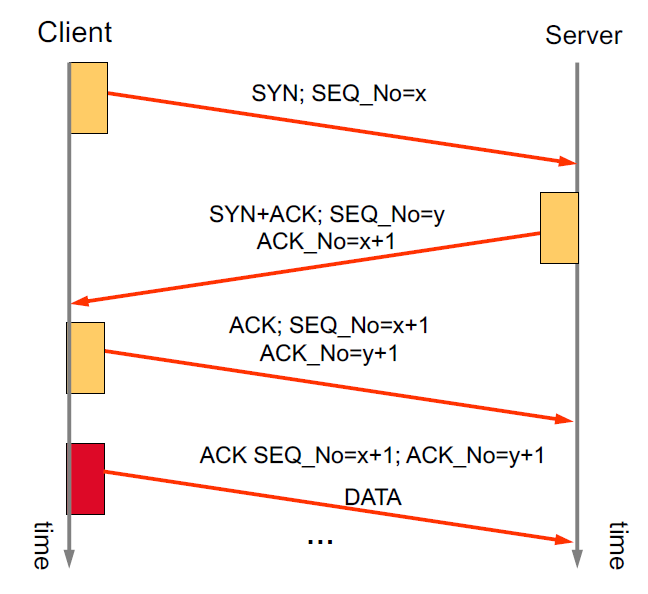
\includegraphics[scale=0.6]{tcp_handshake}
\end{center}

\subsection{Procedura di chiusura di una connessione}

Il \textbf{rilascio di una connessione} in TCP inizia con l'\textbf{invio da parte del client} di un pacchetto contenente il flag \textbf{FIN=1}. Il \textbf{server lo riscontra} inviando \textbf{ACK=1} e poi manda la \textbf{prima mezza chiusura}, ossia un pacchetto con \textbf{FIN=1}. Il \textbf{client riscontra} il segmento \textbf{inviando al server ACK=1}. A questo punto il client potrebbe già chiudere la connessione, ma \textbf{attende} prima di farlo perché potrebbero esserci ancora dei \textbf{segmenti in volo} provenienti dal server. Il tempo di attesa prima della \textbf{seconda mezza chiusura} (che chiude definitivamente la connessione) è di \textbf{2 MSL} (Maximum Segment Lifetime), variabile del sistema operativo personalizzabile. Occorre specificare che durante questo intervallo di attesa non è possibile utilizzare la stessa local port per una nuova connessione. Di seguito lo schema del rilascio connessione realizzato dal docente:

\begin{center}
    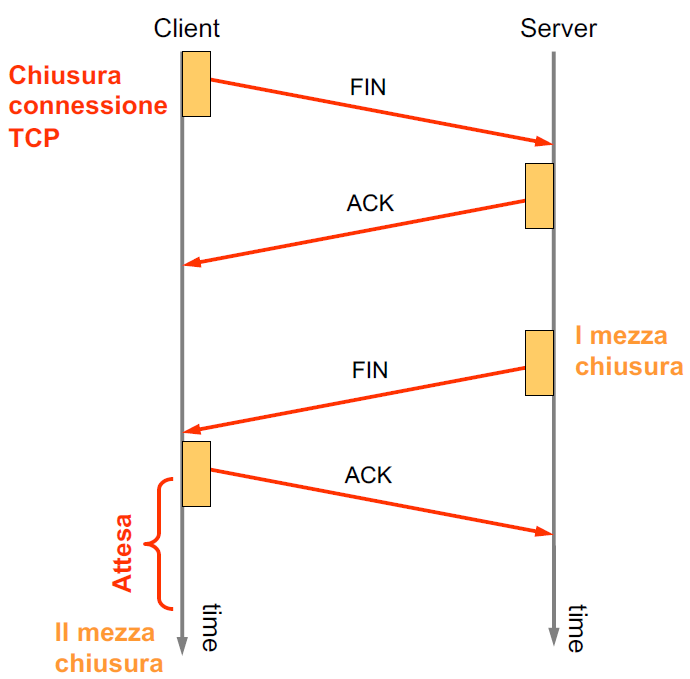
\includegraphics[scale=0.4]{tcp_release}
\end{center}

\subsection{Stati del client}

Inizialmente il client è in stato \textbf{CLOSED}. Quando \textbf{inizializza una connessione} (inviando un SYN e iniziando la procedura di Three-Way Handshake), entra in stato \textbf{SYN\_SENT}. Dopo aver completato la procedura correttamente, entra in stato \textbf{ESTABILISHED}. A questo punto la connessione è stata stabilita e si stanno inviando i segmenti. Alla chiusura, il \textbf{client invia il flag FIN}, andando in stato \textbf{FIN\_WAIT\_1} (prima mezza chiusura). Quando \textbf{riceve l'ACK}, passa in stato \textbf{FIN\_WAIT\_2}. Una volta \textbf{ricevuto FIN e riscontrato}, passa in stato \textbf{TIME\_WAIT}, in cui \textbf{attende} che gli eventuali segmenti in volo arrivino (attesa di \textbf{2 MSL}). Ad attesa conclusa, avviene la seconda mezza chiusura e il client torna in stato \textbf{CLOSED}, chiudendo il giro. Di seguito lo schema degli stati client TCP realizzato dal docente:

\begin{center}
    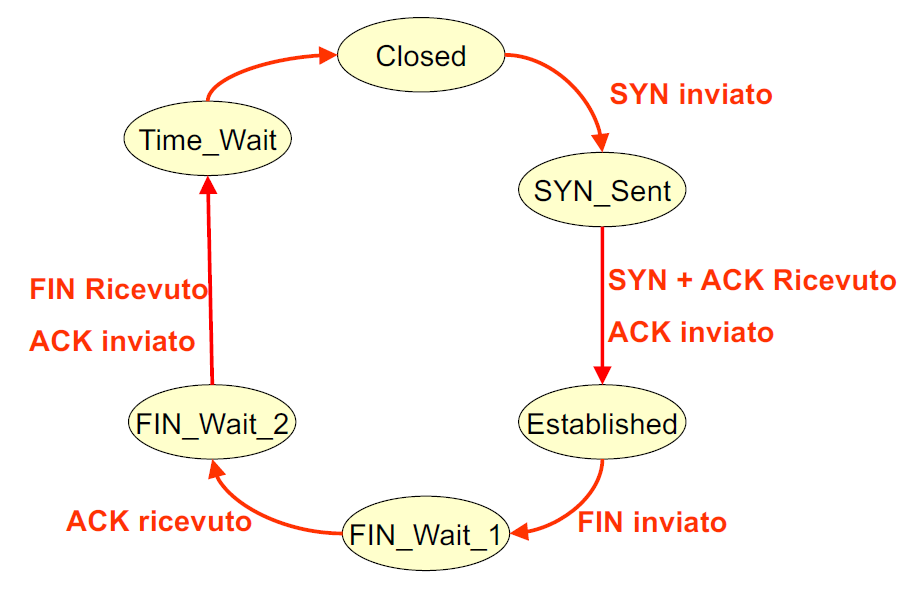
\includegraphics[scale=0.5]{tcp_client_states}
\end{center}

\subsection{Stati del server}

Inizialmente il server è in stato \textbf{CLOSED}. Quando un servizio si mette in ascolto di connessioni in ingresso ad una determinata porta, passa in stato \textbf{LISTEN}. Quando \textbf{riceve} un \textbf{SYN=1 dal client} (richiesta di connessione, che da inizio al Three-Way Handshake), e \textbf{invia SYN=1 e ACK=1}, passa in stato \textbf{SYN\_RCVD}. Quando \textbf{riceve l'ACK dal client}, la connessione è stata stabilita correttamente e passa in stato \textbf{ESTABILISHED}. Durante questo stato avviene la trasmissione dei segmenti. Quando \textbf{riceve un FIN=1} dal client (richiesta di rilascio connessione), e \textbf{invia l'ACK}, passa in stato \textbf{CLOSE\_WAIT}. Una volta \textbf{inviato FIN=1} al client, passa in stato \textbf{LAST\_ACK}, in attesa dell'ACK dal client. Una volta che quest'ultimo viene ricevuto, la connessione può dirsi chiusa e il server torna nuovamente a stato \textbf{CLOSED}. Nel server è presente un piccolo buffer detto \textbf{Backlog Queue} che raccoglie tutte le richieste SYN a cui il server ha risposto SYN+ACK. La dimensione di questo buffer determina quanti flussi contemporanei il server è in grado di gestire. Di seguito lo schema degli stati server TCP realizzato dal docente:

\begin{center}
    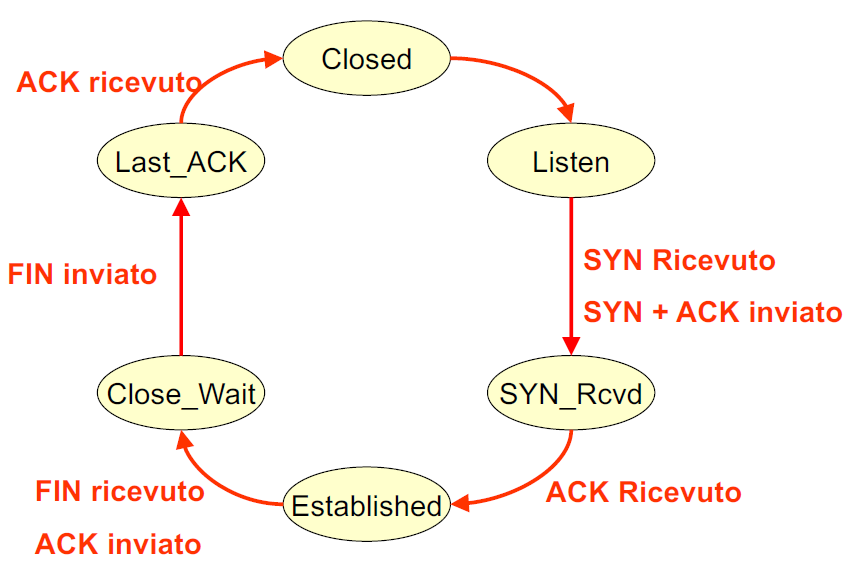
\includegraphics[scale=0.5]{tcp_server_states}
\end{center}

\subsection{Sliding Window}

TCP definisce come \textbf{meccanismo di trasmissione dei segmenti} una finestra \textbf{W} che rappresenta l'\textbf{intervallo di byte} (ossia i segmenti) \textbf{che è possibile inviare contemporaneamente} al receiver. La finestra \textbf{avanza man mano che giungono nuovi ACK} (meccanismo di \textbf{self-clocking}), e la sua dimensione può essere impostata dinamicamente sulla base di algoritmi di controllo di flusso e congestione.

\subsection{RTT e RTO}

L'RTO (\textbf{Retransmission Timeout}) è usato come tempo massimo oltre il quale i segmenti che non sono stati riscontrati sono considerati persi. È possibile calcolare l'RTO dinamicamente sulla base del valore stimato dell'RTT medio. L'RTT (\textbf{Round Trip Time}) è il tempo che intercorre tra l'invio del segmento e la ricezione del suo relativo ACK. Nella pratica, però, si stima l'RTT di un gruppo di diversi segmenti, allo scopo di non memorizzare troppi timeout. Dunque si ha che:
\begin{equation*}
  Transmission\_Rate = \frac{W}{RTT} 
\end{equation*}

\subsection{Stima RTT medio e calcolo RTO}

Per ogni segmento è possibile calcolare un nuovo RTO sulla base del valor medio stimato dell'RTT. Ogni RTT secondi, posso misurare un \textbf{campione} dello stesso RTT, che chiamo $RTT_k$. In questo contesto, RTT è dunque un \textbf{segnale periodico campionato}, di cui si può stimare il valor medio con un \textbf{filtro passa-basso a singolo polo}, cercando di isolare la componente continua dello spettro, valore cui è proporzionale il valor medio.
\begin{align*}
SRTT_k &= a(SRTT_{k-1}) + (1-a)RTT_k\\
DEV_k &= b(DEV_{k-1}) + (1-b)|SRTT_k - RTT_k|\\
RTO_k &= SRTT_k + 4DEV_k
\end{align*}
Un valore comune per $a$ è $\frac{7}{8}$. In seguito a \textbf{timeout successivi}, l'\textbf{RTO viene raddoppiato fino a un determinato numero di volte}. Nei calcoli, $SRTT_k$ rappresenta lo Smoothed RTT, e $DEV_k$ rappresenta la deviazione standard.

\subsection{Controllo di flusso}

Lo scopo del controllo di flusso è di \textbf{evitare la saturazione del buffer di ricezione}. A questo scopo si utilizza il campo \textbf{Advertised Window}, valorizzato nei pacchetti di \textbf{ACK}. Questo valore \textbf{indica lo spazio libero rimanente nel buffer}, dunque viene usato dal mittente come limite superiore per la dimensione della sliding window (W):
\begin{align*}
    AWND &= recv\_buf - (last\_byte\_recvd - last\_byte\_read)\\
    W &= last\_byte\_sent - last\_byte\_acked \leq AWND
\end{align*}

\subsection{Controllo di congestione}

Il controllo di congestione \textbf{regola dinamicamente il rate di trasmissione} dei segmenti al fine di \textbf{utilizzare pienamente la banda disponibile} (si dice che TCP è "\textbf{greedy}"). In contesto TCP è normale avere congestione, anzi si cerca di averla proprio per sfruttare a pieno la banda che si ha a disposizione. Ci sono poi algoritmi atti a gestire le situazioni di congestione in vario modo (TCP Tahoe, Reno e New Reno). \textbf{La congestione avviene a livello 3}, quindi il TCP può solo fare un "guess" sullo stato di congestione, basandosi sul criterio \textbf{3DUPACK} (ricezione di 4 ACK duplicati) o \textbf{scadenza dell'RTO}. Se avviene uno di questi due eventi, TCP banalmente \textbf{riduce W} in modo tale da ridurre i carichi sui buffer dei nodi intermedi posti tra mittente e destinatario e sperare che tutto torni a funzionare. Si usa dunque una variabile detta \textbf{Congestion Window} (CWND) per limitare W:
\begin{equation*}
    W = min(CWND, AWND)
\end{equation*}
Il valore di CWND è gestito da un \textbf{algoritmo di controllo di congestione}.

\subsubsection{Algoritmo generale di controllo congestione}

Tutte le varianti degli algoritmi di controllo congestione (detti "flavor") implementano questi passaggi comuni:
\begin{lstlisting}[language=Octave]
% MSS = Maximum Segment Size, dim. massima del payload
CWND = 1 MSS
% Slow Start Threshold
SS_THRES = MAX % Definito da OS
    
% FASE DI 'PROBING', VOGLIO CAPIRE QUANTA BANDA HO
CWND += 1 MSS % PER OGNI ACK RICEVUTO
% RADDOPPIATA PER OGNI RTT (RISCONTRO INTERA FINESTRA)
    
% SE SI VERIFICA CONGESTIONE
if CONGESTION == TRUE:
    % APPLICO ALGORITMO PER MODIFICARE CWND e SS_THRESH
        
if CWND > SS_THRES:
    % SCATTA CONGESTION AVOIDANCE
    CWND += (1 / CWND) MSS % PER OGNI ACK RICEVUTO
    % OSSIA AUMENTA AL PIU' 1 MSS OGNI RTT
    % A PRESCINDERE DA QUANTI ACK RICEVO
\end{lstlisting}

\begin{center}
    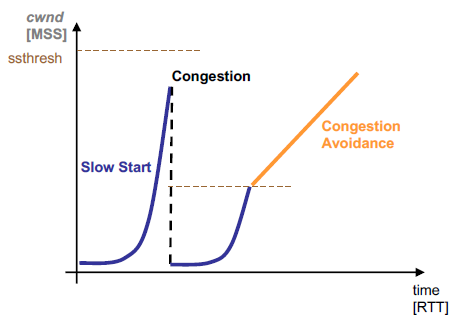
\includegraphics[scale=0.65]{tcp_congestion_algorithm}
\end{center}

\subsubsection{TCP Tahoe}

\begin{lstlisting}[language=Octave]
% ON ACK RECEIVED:
if CWND < SS_THRES:
    CWND += 1 % SLOW START
else
    CWND += (1 / CWND) % CONGESTION AVOIDANCE

% ON 3DUPACK RECEIVED OR TIMEOUT RTO:
SS_THRES = CWND / 2
CWND = 1
\end{lstlisting}
Ha uno svantaggio importante: \textbf{non distingue tra 3DUPACK e TIMEOUT RTO} sebbene quest'ultimo si verifichi in casi più gravi di congestione della rete.

\begin{center}
    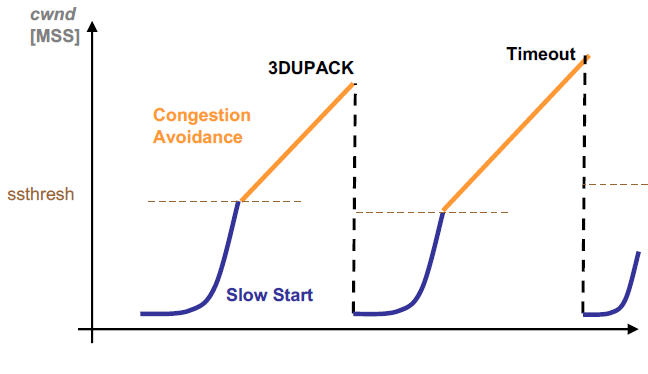
\includegraphics[scale=0.5]{tcp_tahoe}
\end{center}

\subsubsection{TCP Reno}

\begin{lstlisting}[language=Octave]
% ON ACK RECEIVED:
if CWND < SS_THRES:
    CWND += 1 % SLOW START
else
    CWND += (1 / CWND) % CONGESTION AVOIDANCE

% ON 3DUPACK RECEIVED:
SS_THRES = CWND / 2
CWND = SS_THRES % FAST RECOVERY

% ON TIMEOUT RTO: % SAME AS TAHOE
SS_THRES = CWND / 2
CWND = 1
\end{lstlisting}
Sebbene migliore di Tahoe,\textbf{ non protegge da eventuali 3DUPACK molteplici nella stessa finestra di ricezione}. La versione New Reno risolve proprio questo problema.

\begin{center}
    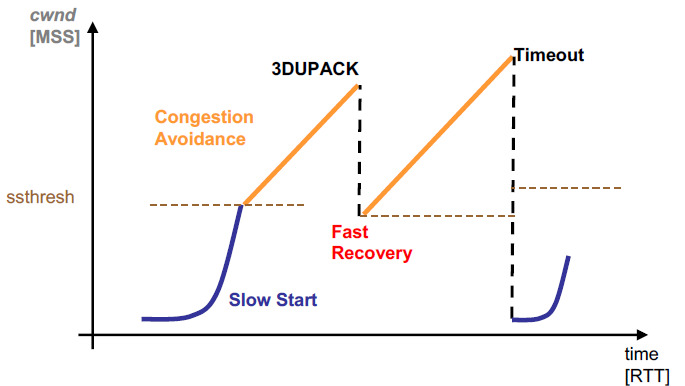
\includegraphics[scale=0.5]{tcp_reno}
\end{center}

\subsubsection{TCP New Reno}

A livello algoritmico è uguale a Reno, ma l'uscita dalla Fast Recovery avviene solo quando si ricevono tutti gli ACK nella finestra di segmenti in volo nel momento di ingresso in Fast Recovery. Questo garantisce un \textbf{throughput migliore nel caso di molteplici 3DUPACK nella stessa finestra di trasmissione}.

\begin{center}
    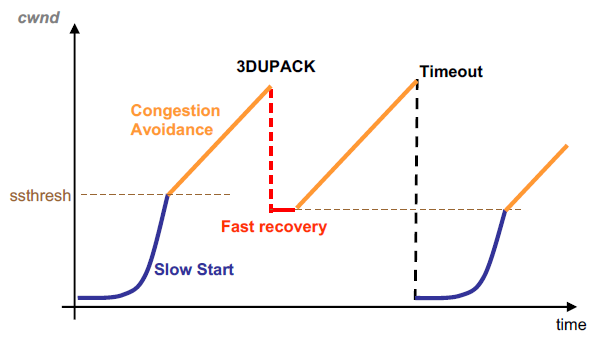
\includegraphics[scale=0.75]{tcp_new_reno}
\end{center}

\subsection{Calcolo del throughput}

Si definisce un semplice modello matematico per analizzare la relazione tra \textbf{throughput} in TCP, \textbf{RTT} e \textbf{probabilità di perdita del segmento P}. In \textbf{condizioni stazionarie} (considerando la perdita di segmenti solo a causa di 3DUPACK) la CWND varia linearmente (1 MSS per RTT) tra il valore di soglia (M/2) e il valore massimo M (retta con pendenza $\frac{1}{RTT}$) con RTT medio ipotizzato costante. Sia T il tempo medio che intercorre tra la perdita di due segmenti. Considerando il coefficiente angolare della retta $\frac{1}{RTT}$ si ha che:
\begin{equation}
    \frac{M - \frac{M}{2}}{T} = \frac{1}{RTT} \Rightarrow M = \frac{M}{2} + \frac{T}{RTT}
\end{equation}
\begin{center}
    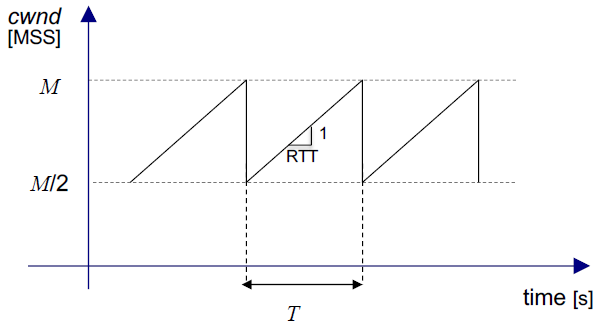
\includegraphics[scale=0.6]{tcp_throughput}
\end{center}
Dunque ottengo un errore ogni T secondi, quindi P = $\frac{1}{N_t}$, dove $N_t$ è il numero di segmenti trasmessi in T secondi. Poiché il rate in TCP è $\frac{W}{RTT}$, allora sostituendo si ottiene $\frac{CWND}{RTT} = r(t)$. Si ha che:
\begin{equation*}
    N_t = \int_{T} r(t) dt
\end{equation*}
L'integrale è pari all'area del trapezio, dunque:
\begin{equation}
    N_t = \frac{T(M + \frac{M}{2})}{2RTT} \Rightarrow P = \frac{1}{N_t} = \frac{2RTT}{T(M + \frac{M}{2})}
\end{equation}
Combinando (1) e (2) si ha che $T = \sqrt{\frac{2}{3P}}RTT$. Poiché il throughput S è dato dal numero di segmenti inviati in T, si ha:
\begin{equation*}
    S = \frac{N_t}{T} = \frac{1}{PT} = \sqrt{\frac{3}{2}}\frac{1}{RTT\sqrt{P}}
\end{equation*}
In conclusione, il throughput in TCP è proporzionale al rapporto $\frac{1}{RTT\sqrt{P}}$. È importante osservare che il \textbf{TCP è robusto agli errori}, in quanto al denominatore è presente una radice quadrata, quindi all'aumentare della probabilità, S diminuisce lentamente.

\section{Domande sul layer IP}

\subsection{Caratteristiche fondamentali del pacchetto IP}

Un flusso di pacchetti IP è sempre identificato da:
\begin{itemize}
    \item IP host mittente
    \item IP host destinatario
    \item Porta locale
    \item Porta remota
    \item Protocollo di trasporto
\end{itemize}

\subsection{Richiesta ARP}

L'\textbf{Address Resolution Protocol} (ARP) è utilizzato per conoscere il \textbf{MAC Address} (identificativo host di livello 2) corrispondente ad un particolare indirizzo IP. Sia A host mittente e B host destinatario (nella stessa rete) di cui si conosce l'IP. A invia una richiesta in broadcast indicando l'IP di B. B, vedendo il suo IP, risponderà ad A in unicast passandogli il suo MAC Address. Ogni host ha una cache che memorizza le risoluzioni più recenti, detta \textbf{ARP Cache}.

\subsection{DHCP}

Il protocollo DHCP (\textbf{Dynamic Host Configuration Protocol}) consente ad un host di ottenere da un DHCP Server: \textbf{IP}, \textbf{netmask}, \textbf{IP del default router}, \textbf{IP del server DNS} e \textbf{lease time} (intervallo di tempo in cui si può usare l'IP assegnatoci, scaduto il quale si dovrà effettuare una nuova richiesta). Si possono avere più server DHCP nella stessa rete, in tal caso l'host sceglierà la risposta che riterrà migliore. Se il server DHCP non è presente nella rete locale, un router della rete locale può avere la funzione di \textbf{DHCP Relay}: esso conosce dove si trova il vero DHCP ed inoltra le richieste DHCP provenienti dagli host della rete locale (facendo essenzialmente finta di essere il vero DHCP Server). Si può ottenere, configurando appropriatamente il server DHCP, anche un \textbf{IP riservato} sulla base del MAC Address per uno o più host. Il funzionamento di DHCP prevede i seguenti passaggi:
\begin{enumerate}
    \item L'host che vuole un IP invia un messaggio \textbf{DHCPDISCOVER} incapsulandolo in UDP (source port 68, destination port 67). La richiesta è inviata in broadcast sulla rete locale (perché l'host non sa dove si trova):
    \begin{itemize}
        \item SOURCE IP: 0.0.0.0 (Host non ha indirizzo)
        \item DESTINATION IP: 255.255.255.255 (Messaggio broadcast)
    \end{itemize}
    \item Tutti i DHCP Server presenti nella rete (o DHCP Relay se nessuno) rispondono in broadcast (in modo che ogni server sia informato di quanto hanno proposto gli altri) con un messaggio \textbf{DHCPOFFER}.
    \item L'host sceglie l'offerta rispondendo con un messaggio \textbf{DHCPREQUEST}.
    \item Il server conferma l'assegnazione con un messaggio \textbf{DHCPACK} in broadcast. Il processo è concluso, l'IP è stato assegnato.
\end{enumerate}

\subsection{NAT}

Il NAT (Network Address Translation) svolge la funzione di \textbf{sostituzione degli IP}. Questa funzionalità viene tipicamente svolta dal \textbf{router di frontiera}. Quando deve inviare pacchetti verso internet, sostituisce l'IP mittente con un altro IP, allo scopo di \textbf{mascherare gli IP privati} e consentire la comunicazione con le reti di internet. Quando arriva un pacchetto da internet, il router di frontiera utilizza la sua \textbf{Translation Table} per selezionare a quale host è diretto il pacchetto. Questa tabella è costruita osservando le coppie IP mittente/Porta dei pacchetti in uscita. Si crea dunque un'associazione statica tra IP privato di un host e IP pubblico (1-1), detto \textbf{NAT Statico}. Esiste anche una variante dinamica che associa ad ogni host una porta, così è possibile utilizzare lo stesso IP pubblico per più host (N-1). Quest'ultimo si dice \textbf{NAT Dinamico}.

\subsection{Zero Configuration Networking}

L'idea è quella di configurare una rete locale in assenza di amministratori di rete, risultando ideale per piccole reti prive di server DHCP e server DNS. Il funzionamento è semplice: a partire da un \textbf{Link Local Address} (169.254.0.0/16, riservato da IANA), si sceglie casualmente (con distribuzione uniforme) un indirizzo nel range [169.254.11.0-169.254.254.254]. I primi e gli ultimi 256 indirizzi sono riservati per usi futuri. Il Random Number Generator per questa scelta casuale è inizializzato con seed MAC Address della scheda di rete. A questo punto si invia un \textbf{ARP PROBE}, ossia una richiesta ARP con destinatario l'IP da testare. Se arriva risposta, si scopre che quell'indirizzo è stato già scelto, quindi se ne sceglie un altro. Se non arriva risposta, l'indirizzo risulta libero e viene annunciato mediante un \textbf{ARP ANNOUNCEMENT}.

\subsection{Ping e Traceroute}

Ping e Traceroute sono degli applicativi che offrono funzionalità utili per un amministratore di rete per ottenere informazioni su una rete al fine di effettuare troubleshooting. Entrambi utilizzano l'\textbf{Internet Control Message Protocol} (ICMP) per inviare i messaggi e ricevere eventuali risposte o errori. \textbf{Ping} utilizza i messaggi \textbf{ECHO REQUEST} (codice ICMP 8-0) e \textbf{ECHO REPLY} (0-0) per controllare se un determinato host risponde correttamente alle richieste in ingresso. Se l'host non è online o è guasto, non risponderà alle richieste e il programma lo segnalerà. Il programma, inoltre, invia multiple richieste all'host destinatario allo scopo di verificare il quantitativo di pacchetti persi, e stimare l'RTT. \textbf{Traceroute} è un altro programma, più avanzato di Ping, che invia all'host destinatario normali datagram IP con TTL crescente (parte da 1, poi 2, 3, 4 etc). Il programma legge i messaggi di errore \textbf{TTL EXPIRED} che arrivano dai router intermedi posti tra mittente e destinatario, in maniera tale da leggerne le informazioni e costruire la strada attraverso i router che i pacchetti percorrono per raggiungere il destinatario. Un router potrebbe essere configurato per non divulgare le sue informazioni quando vede un TTL EXPIRED, così da anonimizzarsi agli occhi di Traceroute. In tal caso il router apparirà come * in output.

\subsection{Invio pacchetti con host A e B nella stessa rete}

Host A effettua la \textbf{AND logica} tra il suo IP e netmask e l'IP del destinatario e netmask (usando la netmask nel caso classless oppure ricavandola basandosi sul valore dei bit più significativi nel caso classful). Se il risultato è lo \textbf{stesso IP di rete}, significa che i due host sono sulla stessa rete, quindi è possibile comunicare direttamente a livello 2. Se non si conosce il MAC Address di B, A effettua una \textbf{richiesta ARP}.

\subsection{Invio pacchetti con host A e B in reti differenti}

Host A effettua la \textbf{AND logica} tra il suo IP e netmask e l'IP del destinatario e netmask (usando la netmask nel caso classless oppure ricavandola basandosi sul valore dei bit più significativi nel caso classful). Se il risultato sono \textbf{IP di rete differenti}, significa che i due host sono su reti diverse, quindi \textbf{A si rivolge al suo default gateway} (router che connette la rete locale all'esterno). A deve conoscere l'IP del default gateway (configurandolo a mano o mediante DHCP). \textbf{A invia una richiesta ARP per conoscere il MAC Address del default gateway} (se necessario). Infine, \textbf{A invia il pacchetto IP al default gateway}, che si occuperà di instradarlo con le reti internet. In questo contesto viene anche applicato il NAT, mascherando l'IP del mittente e rimpiazzandolo con l'IP pubblico per la comunicazione verso internet.

\subsection{Distance Vector}

Periodicamente, il router invia ai suoi vicini il suo \textbf{vettore delle distanze}, ossia un insieme di righe ottenuto prendendo (dalla sua tabella di routing) la colonna delle \textbf{destinazioni conosciute} e i \textbf{relativi costi}. I router utilizzano queste informazioni per scoprire percorsi migliori e aggiornare la propria tabella di routing. I router memorizzano le destinazioni esistenti e i loro costi \textbf{senza conoscere l'intero grafo della rete}. Dopo un certo \textbf{tempo di convergenza}, tutti i router della rete si conosceranno. Il problema è che questo tempo di convergenza diventa \textbf{molto elevato in reti di grandi dimensioni}, il che può portare a inconsistenze con conseguenti \textbf{problemi di routing loop} causati dal cambiamento topologico della rete prima della convergenza del Distance Vector. Per reti piccole, invece, il tempo di convergenza è relativamente breve, quindi si riducono le probabilità di inconsistenze.

\subsubsection{Algoritmo di Bellman-Ford}

In Distance Vector, il comportamento di scambio delle informazioni tra un router e l'altro realizza di fatto l'\textbf{algoritmo di Bellman-Ford} applicato a un grafo di cui si conosce l'intera topologia. Il \textbf{Distance Vector non implementa davvero questo algoritmo}, ma l'algoritmo è quello che matematicamente rappresenta il comportamento del Distance Vector. Si parte da un generico nodo S nel grafo, e si definiscono:
$D^h_j$ costo del cammino minimo tra S e nodo j con massimo h salti; $d_{ij}$ costo del collegamento diretto tra i e j ($\infty$ se i nodi non sono connessi direttamente). I passaggi dell'algoritmo sono:
\begin{align*}
    (1): h &= 0; D^h_j = \infty, \forall j \neq s, D_s = 0\\
    (2): h &= h + 1; D^h_j = min(D^{h-1}_i + d_{ij}, D^{h-1}_j)\\
    (3): if\ D^h_j &== D^{h-1}_j, \forall j \neq s\ \Rightarrow\ h_{MAX} = h - 1;\  STOP;\ else\ \Rightarrow\ goto\ (2)
\end{align*}

\subsection{Soluzioni del routing loop nel Distance Vector}

Il problema del routing loop nel Distance Vector può essere risolto adoperando una variante del Distance Vector chiamata \textbf{Split Horizon}: il router \textbf{non manderà al suo vicino ciò che il vicino stesso gli ha insegnato}. Si può anche andare oltre con un'ulteriore variante, \textbf{Split Horizon with Poison Reverse}: in questo caso il router \textbf{manda al vicino anche ciò che il vicino gli ha insegnato, ma con costo infinito}. In questo modo il vicino sa che il nodo non conosce realmente la destinazione, ma sa che l'ha imparata da lui. In aggiunta a una di queste due strategie (che sono mutualmente esclusive) si può aggiungere il \textbf{Trigger Update}: quando vi è un cambiamento topologico nella rete (nodo guasto o spento), faccio scattare immediatamente la procedura di invio del Distance Vector, in modo da contrastare la formazione di routing loops.

\subsection{Routing Information Protocol}

Il \textbf{Routing Information Protocol} (RIP) è \textbf{adatto a reti piccole}, usa come algoritmo di routing il \textbf{Distance Vector} e come metrica gli hop count. \textbf{Max hop count = 15}, quindi 16 rappresenta il nodo non raggiungibile ($\infty$). Definisce, dunque, un vero e proprio \textbf{limite superiore alla dimensione della rete} (causato dai massimi salti possibili pari a 15). Routing Update avviene ogni 30 secondi, in più c'è il Trigger Update. Hold-down Timer pari a 120 secondi. Ne esistono 2 versioni: la seconda è più moderna e cambia il formato dei pacchetti introducendo un basilare metodo di autenticazione. Si utilizza UDP a livello 4 per lo scambio dei messaggi RIP sulla porta 520, ogni messaggio contiene fino a 25 descrittori di route. Il RIPv2 trasmette anche la subnet mask dell'indirizzo associato, usa il Route Tag per differenziare route interne ed esterne e il Next Hop per indicare un router diverso da chi ha mandato il messaggio.

\subsection{Link State}

Periodicamente, \textbf{ogni router invia a tutti gli altri router della rete le informazioni relative al costo dei collegamenti con i propri vicini}. L'effetto finale è che tutti i router possono costruire nella loro memoria l'\textbf{intero grafo della rete} con tutti i costi in brevissimo tempo. Conoscere l'intera topologia della rete rende i router in grado di applicare un algoritmo di risoluzione dei grafi per il calcolo del cammino più breve e meno costoso. Il più famoso e utilizzato è l'\textbf{algoritmo di Dijkstra}. Il periodo di aggiornamento è molto più lungo di Distance Vector (anche 30 minuti) a patto che ci sia Trigger Update. Link State risulta \textbf{più efficiente in reti grandi}, ma va gestito correttamente in quanto il costo computazionale di Dijkstra potrebbe rivelarsi elevato.

\subsubsection{Algoritmo di Dijkstra}

Partendo da un generico nodo S, si pone: $D_j$ costo del cammino a costo minimo da s a j; $d_{ij}$ costo di collegamento diretto tra i e j, con valore $\infty$ se i nodi non sono connessi direttamente; N insieme dei nodi della rete e M insieme dei nodi dell'albero corrente, sottoinsieme di N; V(M) insieme dei nodi adiacenti all'insieme M raggiungibili con un singolo hop da un qualunque nodo di M.
\begin{align*}
    (1)\ Init&: M = \{S\},\ D_j = d_{sj}\ \forall j \in V(s) \quad otherwise \quad D_j = \infty\\
    (2)\ Select&: K \in V(S)\ |\ D_k = min_{i \in V(M)}\{D_i\}\\
    &\ \ M = M\ \cup\ \{K\}\\
    &\ \ D_j = min(D_j,\ D_k + d_{kj})\ \forall j \in V(M)\\
    (3)\ If&: M == N \Rightarrow STOP;\ else\ goto\ (2)
\end{align*}

\subsection{Protocollo OSPF}

Il protocollo OSPF (\textbf{Open Shortest Path First}) è adatto a reti di grandi dimensioni, utilizza il \textbf{Link State} come algoritmo di routing e si occupa di \textbf{implementare il flooding concettuale} visto in quest'ultimo (che non è applicabile nella realtà nel mondo IP) \textbf{sfruttando gli indirizzi IP multicast riservati} (di classe D). Ogni router ha un suo \textbf{Router ID}, incluso negli \textbf{Hello Packet} inviati periodicamente su tutte le interfacce (in LAN si usa l'indirizzo multicast 224.0.0.5). \textbf{Possono essere usate tutte le metriche} per ognuno dei servizi previsti dal campo ToS, dunque è molto più flessibile di RIP che invece limita le metriche usabili al solo hop count. \textbf{Ogni AS è diviso in aree} ognuna definita da 4 otetti in una \textbf{struttura gerarchica}. Allo scopo di implementare il flooding concettuale, periodicamente ogni nodo invia lo stato dei suoi collegamenti in un \textbf{Link State Packet (LSP)}. In OSPF, ogni LSP contiene più \textbf{Link State Advertisement (LSA)} che specificano lo \textbf{stato dei singoli link}. Se un router vuole comunicare con un router in un'altra area, dovrà per forza passare attraverso la \textbf{Backbone Area} (con ID 0) mediante gli \textbf{Area Border Router}, che segnala al router originale di essere collegato al destinatario (fittiziamente), riceve il pacchetto IP e poi mediante un suo albero lo manda all'Area Border Router dall'altro lato, che poi lo rimanderà al destinatario. In definitiva \textbf{tutte le comunicazioni inter-area passano attraverso la backbone}.

\subsection{Border Gateway Protocol}

Definisce \textbf{quali sono gli AS raggiungibili da un dato AS, e la strada tra AS per raggiungerli}. Ci sono diversi tipi di AS:
\begin{itemize}
    \item \textbf{STUB}: Il router del border gateway è collegato in uscita con un solo AS;
    \item \textbf{MULTIHOMED}: Il gateway ha più uscite verso molteplici AS;
    \item \textbf{TRANSIT}: Collegato a più AS e trasporta traffico da AS diversi.
\end{itemize}
Tra due router di bordo si stabilisce una \textbf{connessione TCP} sulla porta 179 (si parla di Peer BGP Router). Si potrebbe usare BGP anche per comunicazioni intra-AS (anche se non è usato, si preferisce optare per RIP o OSPF): in tal caso si parla di \textbf{Interior BGP Session}, altrimenti \textbf{Exterior} (com'è di solito). I router di bordo hanno la loro tabella di routing arricchita con la sequenza di AS da attraversare per ogni rete, detta \textbf{Path Vector}. Ogni router annuncia le diverse reti usando il \textbf{CIDR}, quindi eventualmente raggruppando gli indirizzi per compattare e risparmiare dati. Questo annuncio, detto \textbf{Route}, contiene i \textbf{Prefix} (IP di rete in CIDR) e gli \textbf{Attributes} che offrono ulteriori informazioni. Gli Attributes più importanti sono:
\begin{itemize}
    \item \textbf{AS-PATH}: Elenco degli AS attraverso cui è passato l'annuncio del Prefix;
    \item \textbf{NEXT-HOP}: Scelta del nodo successivo nel caso vi siano più route per un Prefix.
\end{itemize}
Un router può accettare o meno gli annunci che gli giungono in base alle sue \textbf{policy}. Viene scelto l'\textbf{AS-PATH più breve come metrica} per instradare il pacchetto.

\section{Domande sul layer Data Link}

\subsection{Protocollo Stop \& Wait}

Nel protocollo Stop \& Wait, \textbf{il mittente invia la trama e si ferma (STOP), attendendo (WAIT) il riscontro} (ossia un pacchetto di ACK molto piccolo) dal destinatario. Quest'ultimo controlla eventuali errori e, se tutto è corretto, invia l'ACK quando ha terminato di processare il pacchetto. Il mittente riceve l'ACK che attendeva, effettua l'error check, e infine è sicuro che i dati sono arrivati, dunque scarta il frame dal buffer di ritrasmissione. Se così non fosse andata, \textbf{dopo un certo periodo} $T_{OUT}$, il mittente avrebbe \textbf{rinviato lo stesso pacchetto} rimettendosi in attesa.
\begin{center}
    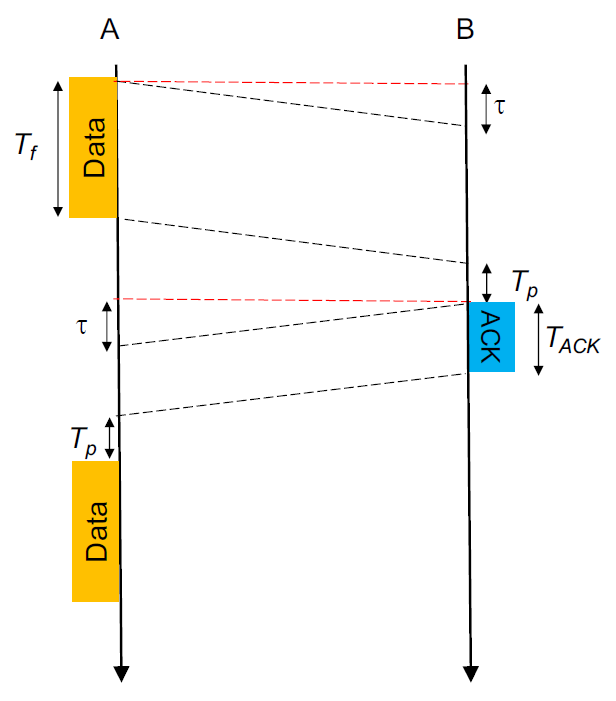
\includegraphics[scale=0.3]{stop_and_wait}
    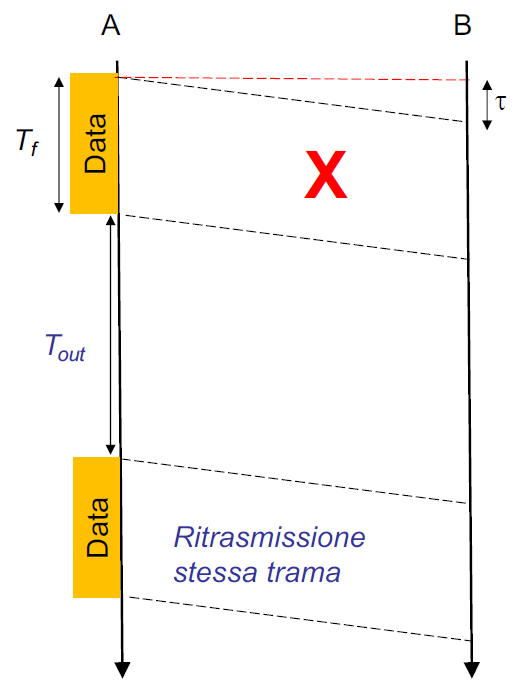
\includegraphics[scale=0.3]{stop_and_wait_with_timeout}
\end{center}

\subsection{Efficienza in Stop \& Wait}

\subsubsection{In assenza di errore (P = 0)}

In Stop \& Wait, il \textbf{tempo necessario a trasferire una trama} è:
\begin{equation*}
    T_{TOT} = T_f + T_{ACK} + 2T_P + 2\tau
\end{equation*}
Dove $T_f$ è il \textbf{tempo di trasmissione della trama} (componente \textbf{utile}), $T_{ACK}$ è il \textbf{tempo di trasmissione del riscontro}, $T_P$ è il \textbf{tempo di elaborazione} della trama (dal ricevente), e $\tau$ è il \textbf{tempo di propagazione} (dipende dal mezzo di trasmissione). Queste ultime 3 componenti caratterizzano il \textbf{ritardo}. L'\textbf{efficienza}, in generale, si calcola come:
\begin{equation*}
    \eta = \frac{T_f}{T_{TOT}}
\end{equation*}
Il valore ideale di $\eta$ è 1. Considerando che $T_{ACK}$ e $T_P$ \textbf{sono molto piccoli rispetto a} $T_f$, l'espressione di $T_{TOT}$ si può semplificare:
\begin{equation*}
    T_{ACK},\ T_P \ll T_f\ \Rightarrow\ T_{TOT}\ \cong\ T_f + 2\tau
\end{equation*}
Sostituendo nell'espressione dell'efficienza:
\begin{equation*}
    \eta\ \cong\ \frac{T_f}{T_f + 2\tau}\ =\ \frac{1}{1 + 2a},\ a\ =\ \frac{\tau}{T_f}
\end{equation*}
Dove $a$ è il \textbf{ritardo di propagazione normalizzato}. Il \textbf{throughput} è dunque pari a $\eta$C dove \textbf{C} è la \textbf{frequenza di cifra} (banda disponibile nel canale). \textbf{Anche in assenza di errori, in S\&W $\eta$ non è mai unitaria}.

\subsubsection{In presenza di errore (P $\neq$ 0)}

Ora ricaviamo l'efficienza in S\&W in caso di errori. Nel protocollo, \textbf{il mittente aspetta un certo timeout prima di rinviare} il frame automaticamente. Se il frame dovesse \textbf{arrivare al destinatario errato}, infatti, questo \textbf{viene scartato senza l'invio dell'ACK} (dunque scadrà il timeout del mittente). Necessariamente deve essere che:
\begin{equation*}
    T_{OUT}\ \geq\ T_{ACK} + 2T_P + 2\tau
\end{equation*}
In questo caso \textbf{l'efficienza dipende dal numero di trasmissioni dello stesso frame} (che denotiamo $N_s$) prima della ricezione di un ACK corretto. Ovviamente se $N_s$ è piccolo (caso limite 1, in quel caso non ci sono stati errori) l'efficienza aumenta. Aggiungendo le ritrasmissioni all'espressione di $T_{TOT}$ si ottiene:
\begin{equation*}
    T_{TOT}\ =\ (N_s - 1)(T_f + T_{OUT}) + T_f + T_{ACK} + 2T_P + 2\tau
\end{equation*}
$N_s$ in questo contesto è una \textbf{variabile aleatoria}, in quanto dipende dagli errori sul canale, quindi occorre considerarne il \textbf{valor medio}, e per conoscerlo occorre conoscere la \textbf{distribuzione}, che dipende dal \textbf{BER (Bit Error Rate)}. Sia \textbf{P} la \textbf{probabilità di errore su un singolo bit}. Si ipotizza il \textbf{CBS (Canale Binario Simmetrico)}, cioè errori sui bit indipendenti tra loro (che è il caso peggiore, in quanto così gli errori sono davvero imprevedibili). Siano $L_f$ e $L_{ACK}$ le lunghezze in bit di trama dati e trama ACK. Data l'ipotesi di indipendenza, il \textbf{FER (Frame Error Rate)} sarà calcolato come complemento della probabilità di trasmissione della trama con successo:
\begin{equation*}
    1 - FER\ =\ (1 - P)^{(L_f + L_{ACK})}\ \Rightarrow\ P\ =\ FER\ =\ 1 - (1 - P)^{(L_f + L_{ACK})}
\end{equation*}
Ora è possibile determinare la distribuzione di $N_s$:
\begin{align*}
    N_s = 1\ &\Rightarrow\ pr\{N_s = 1\}\ =\ 1 - P\\
    N_s = 2\ &\Rightarrow\ pr\{N_s = 2\}\ =\ P(1 - P)\\
    N_s = 3\ &\Rightarrow\ pr\{N_s = 3\}\ =\ P^2(1 - P)\\
    ...\\
    N_s = k\ &\Rightarrow\ pr\{N_s = k\}\ =\ P^{k-1}(1 - P)
\end{align*}
Si nota la costante presenza di $1-P$ a rappresentare proprio la \textbf{prima trasmissione}. Il resto sono \textbf{ritrasmissioni dovute a errori}. Ora è possibile calcolare il valor medio della distribuzione con il metodo classico:
\begin{equation*}
    \overline{N_s}\ =\ \sum^{+\infty}_{k=1}kP^{k-1}(1-P)\ =\ (1-P)\sum^{+\infty}_{k=1}kP^{k-1} \ =\ (1-P)\frac{1}{(1-P)^2}\ =\ \frac{1}{1-P}
\end{equation*}
Si nota facilmente la presenza della \textbf{derivata della serie geometrica} che da' come risultato $\frac{1}{(1-P)^2}$, permettendoci di semplificare la distribuzione. Ora è possibile calcolare l'efficienza:
\begin{equation*}
    \eta\ =\ \frac{T_f}{T_{TOT}}\ =\ \frac{T_f}{(\overline{N_s}-1)(T_f + T_{OUT}) + T_f + T_{ACK} + 2T_P + 2\tau}
\end{equation*}
Trascurando, come prima, i tempi di elaborazione e riscontro (piccoli rispetto a $T_f$), e considerando il minimo valore teorico per il timeout, si ha:
\begin{equation*}
    T_{OUT}\ \cong\ 2\tau\ \Rightarrow\ \eta\ \cong\ \frac{T_f}{(\overline{N_s}-1)(T_f + 2\tau) + T_f + 2\tau}\ =\ \frac{T_f}{\overline{N_s}(T_f + 2\tau)}\ =\ \frac{(1 - P)T_f}{T_f + 2\tau}
\end{equation*}
Andando a sostituire nell'espressione $a$, ossia il ritardo di propagazione normalizzato, si ha l'espressione finale:
\begin{equation*}
    \eta\ =\ \frac{1 - P}{1 + 2a}
\end{equation*}
Ovviamente \textbf{se P = 0 si ritorna al caso precedente}. Considerando questa espressione si nota che, fissato il FER (dipendente dalla rumorosità del canale), \textbf{l'efficienza dipende dal valore del ritardo di propagazione normalizzato}. Ora, considerando la distanza d e la velocità di propagazione delle onde nel mezzo v, si ha:
\begin{equation*}
    a\ =\ \frac{\tau}{T_f}\ =\ \frac{\frac{d}{v}}{\frac{L_f}{C}}\ =\ \frac{dC}{vL_f}
\end{equation*}
\textbf{Stop \& Wait}, pertanto, \textbf{è efficiente in canali lenti} (con bassa frequenza di cifra) o \textbf{collegamenti vicini} (valore di d basso) e \textbf{trame abbastanza grandi} (ma non troppo, altrimenti P aumenta). Questo è proprio il caso d'uso ideale per un \textbf{canale radio}.
Infatti questo protocollo è \textbf{usato} proprio \textbf{da WLAN}!

\subsection{Protocollo Go Back N}

Il protocollo \textbf{Go Back N (GBN)} è di tipo \textbf{Continuous ARQ} (\textbf{Automatic Repeat reQuest}), dunque \textbf{è possibile trasmettere più trame in sequenza mentre si attende il riscontro delle altre}, con meccanismo a \textbf{sliding window} (con necessario meccanismo di numerazione). \textbf{In GBN la finestra di ricezione è sempre unitaria} ($W_R=1$): non richiede, quindi, il riordino dei frame in ricezione. La finestra di trasmissione ($W_S$) stabilisce quante e quali trame inviare di seguito in attesa dei riscontri delle precedenti. Per ogni trama ricevuta correttamente, il ricevitore fa scorrere la finestra di ricezione e invia un \textbf{ACK di tipo cumulativo}: l'i-esimo ACK indica che si sono ricevute correttamente tutte le trame fino alla i-esima. Alla ricezione corretta dell'ACK, il mittente può far scorrere in avanti la sua finestra di trasmissione e inviare la trama successiva. È importante notare che \textbf{in questo protocollo si può avere efficienza senza errori pari a 1}.

\begin{center}
    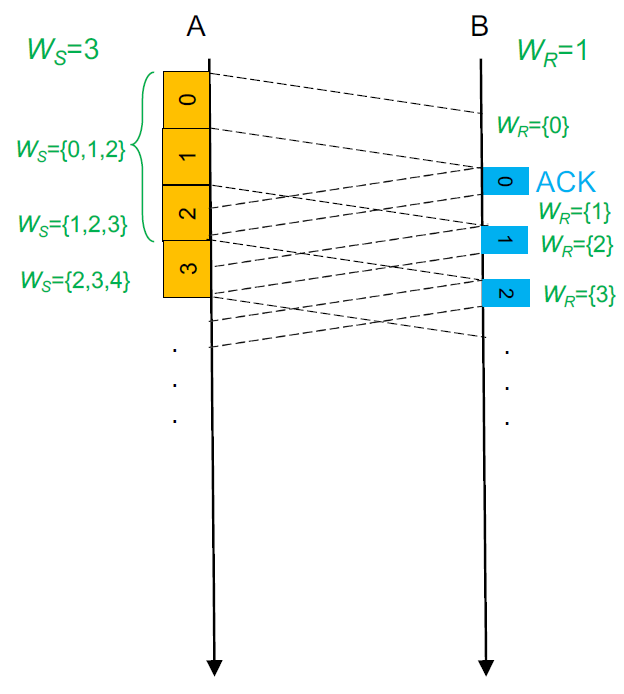
\includegraphics[scale=0.3]{go_back_n}
\end{center}

\subsubsection{Con errore sulla trama}

Nel caso di errore sulla trama, quest'ultima viene scartata, e \textbf{il ricevitore si accorge di averla mancata}, quindi manda al mittente un \textbf{NACK (Negative ACK)} per informarlo dell'evento. Il mittente "\textbf{torna indietro}" (Go Back NACK) \textbf{fino a NACK} e riprende la trasmissione normalmente. Il ricevitore, intanto, scarta le trame successive e attende che gli arrivino nuovamente, ripetendo il processo nel caso di nuovo errore, altrimenti
sarà riscontrata anche la trama per cui si era inviato il NACK e la trasmissione continua con nuove trame. Tutto questo, ovviamente, funziona solo nell'ipotesi di errore solo sulla trama, supponendo che le trame di ACK e NACK siano prive di errori.

\begin{center}
    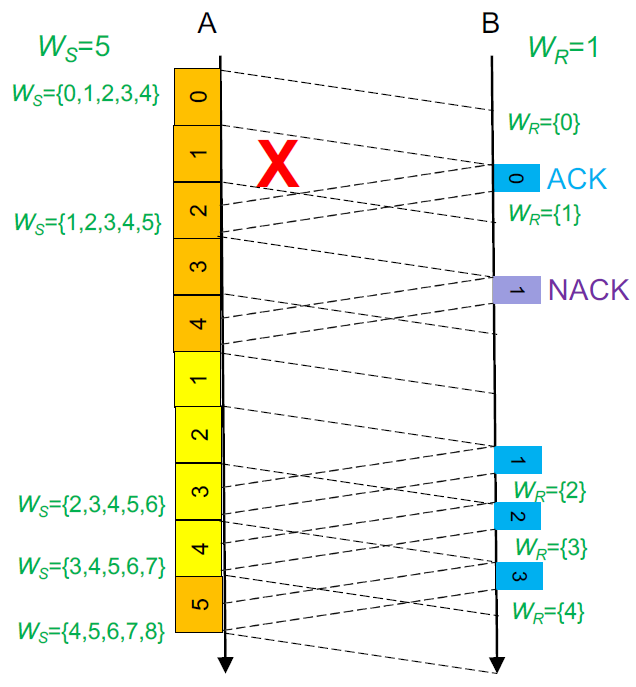
\includegraphics[scale=0.3]{go_back_n_frame_error}
\end{center}

\subsubsection{Con errore sul riscontro}

Al fine di evitare che il sistema si blocchi \textbf{viene avviato un timeout per ogni trama inviata}, scaduto il quale il mittente torna indietro fino alla trama per cui non ha ricevuto l'ACK. Con questa soluzione, tuttavia, sorge il problema dell'\textbf{equivocazione}: \textbf{il ricevente considera come trame nuove delle trame in realtà ritrasmesse} a causa della scadenza del timeout, causato dalla situazione in cui tutti gli ACK che il ricevitore mandava (fino a tornare a $W_R=\{0\}$) non sono arrivati. Quindi il ricevitore pensa di star ricevendo nuove trame, quando invece sono di fatto \textbf{replicate}. \textbf{Per risolvere}, basta mettere come \textbf{limite superiore della finestra di trasmissione N-1 invece di N}. In questo modo, è possibile individuare queste incongruenze.

\begin{center}
    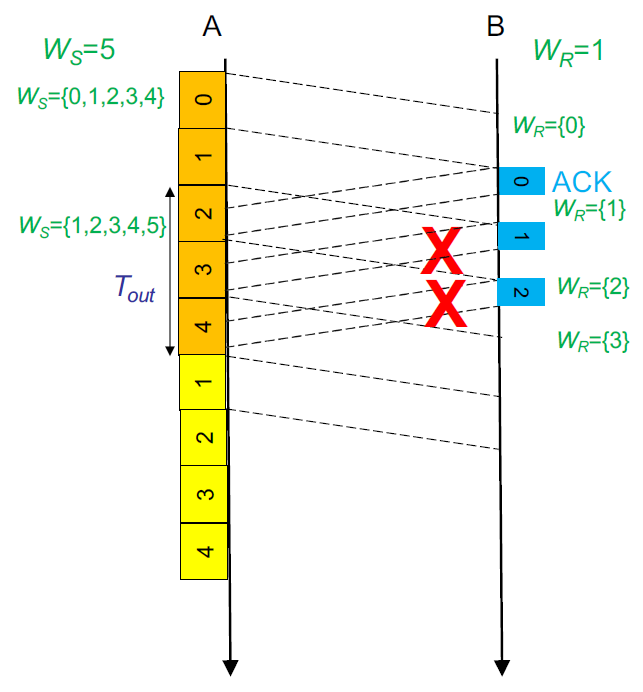
\includegraphics[scale=0.3]{go_back_n_ack_error}
    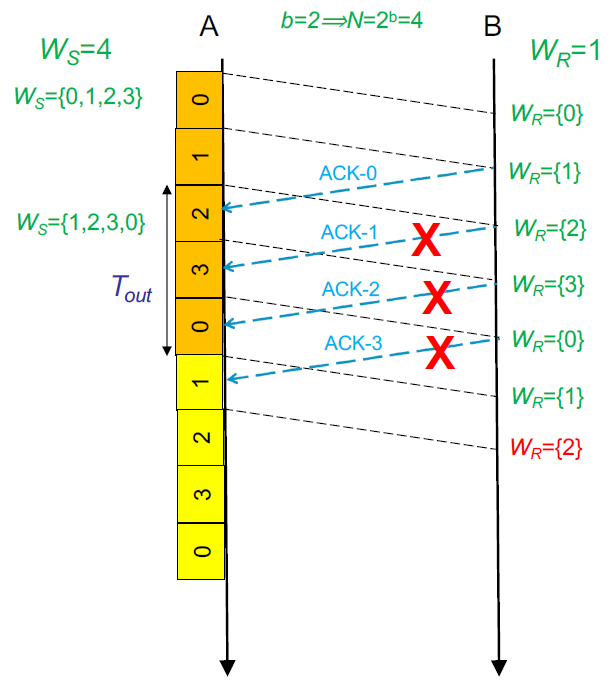
\includegraphics[scale=0.3]{go_back_n_equivocation}
\end{center}

\subsection{Efficienza in Go Back N}

Si suppone che i \textbf{riscontri arrivino nella stessa finestra di trasmissione} e che l'eventuale trama sbagliata sia sempre la stessa. Si trascurano (come prima) i tempi di elaborazione e trasmissione dell'ACK. Si vuole caratterizzare il tempo totale di trasmissione. È evidente che il tempo per trasmettere il frame i è la somma di tutti i tempi delle K trame ripetute fino alla i-esima. Dunque:
\begin{align*}
    N_s\ &=\ num\_errori \cdot K\ +\ 1\\
    T_{TOT}\ &=\ \overline{N_s} \cdot T_f\ \Rightarrow\ \eta\ =\ \frac{T_f}{T_{TOT}}\ =\ \frac{T_f}{\overline{N_s} \cdot T_f}\ =\ \frac{1}{\overline{N_s}}
\end{align*}
Ora, come prima, occorre valutare la distribuzione di $N_s$ per calcolarne il valor medio:
\begin{align*}
    N_s = 1\ &\Rightarrow\ pr\{N_s = 1\}\ =\ 1 - P\\
    N_s = K + 1\ &\Rightarrow\ pr\{N_s = K + 1\}\ =\ P(1 - P)\\
    N_s = 2K + 1\ &\Rightarrow\ pr\{N_s = 2K + 1\}\ =\ P^2(1 - P)\\
    ...\\
    N_s = iK + 1\ &\Rightarrow\ pr\{N_s = iK + 1\}\ =\ P^i(1 - P)
\end{align*}
Dunque il valor medio si calcola come:
\begin{align*}
    \overline{N_s} &= \sum^{+\infty}_{i=0}(iK + 1)P^i(1 - P) = (1 - P)\left[\sum^{+\infty}_{i=0}iKP^i + \sum^{+\infty}_{i=0}P^i\right]=\\&= (1 - P)\left[KP\sum^{+\infty}_{i=1}iP^{i-1} + \frac{1}{1-P}\right] = (1-P)\left[\frac{KP}{(1-P)^2} + \frac{1}{1-P}\right]=\\&= \frac{1 + P(K - 1)}{1 - P}\ \Rightarrow\ \eta = \frac{1}{\overline{N_s}} = \frac{1-P}{1+P(K -1)}
\end{align*}
Si nota che, inoltre, che:
\begin{equation*}
    KT_f\ \cong\ 2T_f + 2\tau\ \Rightarrow\ K\ =\ 2 + 2a
\end{equation*}
Sostituendo, infine, si ha l'espressione finale dell'efficienza in GBN:
\begin{equation*}
    \eta\ =\ \frac{1-P}{1+P(1 + 2a)}
\end{equation*}

\subsection{Protocollo Selective Repeat}

A differenza di GBN, in \textbf{Selective Repeat (SR)} \textbf{anche la finestra di ricezione può essere $>$ 1}. Possono essere, quindi, ricevute \textbf{trame potenzialmente non in ordine} ed è compito del ricevente riordinarle. \textbf{Occorre un buffer anche in ricezione}. L'ACK, come in GBN, è cumulativo. Supponendo di avere un \textbf{errore sulla trama}, qui \textbf{non serve scartare tutte le trame ricevute dopo}, perché posso memorizzarle nella finestra. In caso di errore, il \textbf{NACK informa selettivamente il mittente} su quale frame deve rinviare. Nel caso di \textbf{errori sul riscontro}, ci può comunque essere \textbf{equivocazione}, \textbf{risolvibile evitando che le due finestre si sovrappongano}, ossia riducendo la dimensione delle finestre in modo che la loro \textbf{somma non superi N}.

\begin{center}
    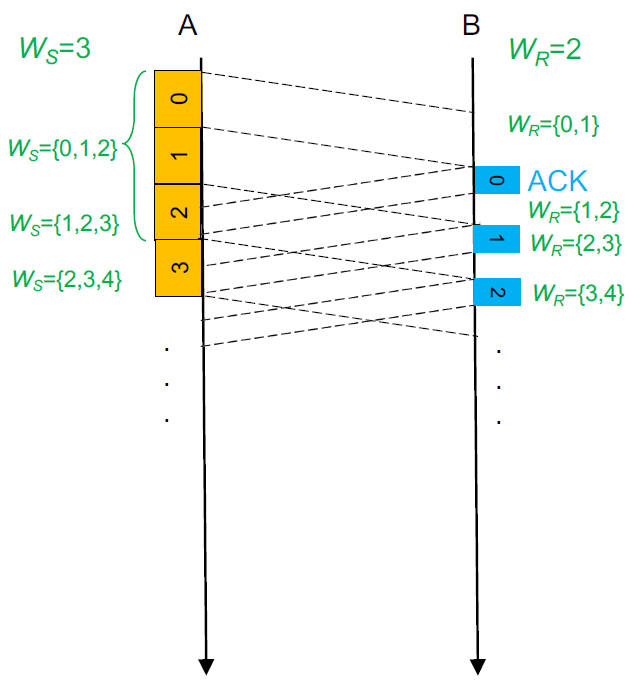
\includegraphics[scale=0.2]{selective_repeat}
    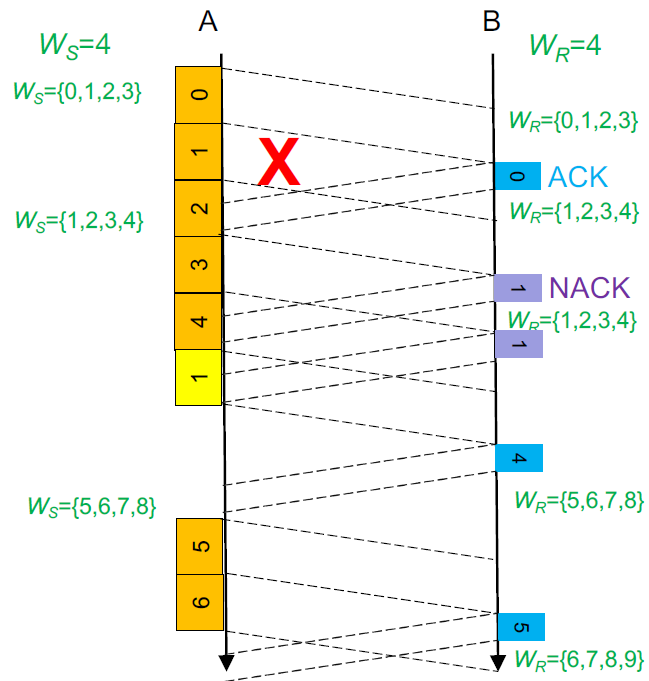
\includegraphics[scale=0.2]{selective_repeat_frame_error}
\end{center}

\subsection{Efficienza in Selective Repeat}

In SR, \textbf{in presenza di errore si ritrasmette solo una trama}, quindi il numero di trasmissioni è:
\begin{equation*}
    N_s = num\_errori + 1
\end{equation*}
L'efficienza risulta uguale a GBN:
\begin{equation*}
    \eta = \frac{T_f}{T_{TOT}} = \frac{T_f}{\overline{N_s} \cdot T_f} = \frac{1}{\overline{N_s}}
\end{equation*}
Ora è possibile calcolare la distribuzione di $N_s$:
\begin{align*}
    N_s = 1\ &\Rightarrow\ pr\{N_s = 1\}\ =\ 1 - P\\
    N_s = 2\ &\Rightarrow\ pr\{N_s = 2\}\ =\ P(1 - P)\\
    N_s = 3\ &\Rightarrow\ pr\{N_s = 3\}\ =\ P^2(1 - P)\\
    ...\\
    N_s = k\ &\Rightarrow\ pr\{N_s = k\}\ =\ P^{k-1}(1 - P)
\end{align*}
Ci si rende conto che \textbf{il risultato è identico a quello ottenuto in S\&W}. Infatti anche il valor medio è precisamente lo stesso:
\begin{equation*}
    \overline{N_s}\ =\ \sum^{+\infty}_{k=1}kP^{k-1}(1-P)\ =\ (1-P)\sum^{+\infty}_{k=1}kP^{k-1} \ =\ (1-P)\frac{1}{(1-P)^2}\ =\ \frac{1}{1-P}
\end{equation*}
Ma stavolta ciò che \textbf{cambia} è \textbf{l'espressione dell'efficienza}. Infatti:
\begin{equation*}
    \eta = \frac{1}{\overline{N_s}} = 1-P
\end{equation*}
Si nota l'\textbf{assenza del ritardo di propagazione normalizzato $a$}, e si vede chiaramente che SR ha l'\textbf{efficienza più elevata} tra tutti i 3 protocolli analizzati, ma è quello con la \textbf{maggiore complessità} (costi più elevati di implementazione per la presenza dei due buffer, uno in trasmissione e uno in ricezione) e per la necessità di gestire il riordinamento dei frame. Non considerando gli errori (P=0), sia GBN che SR hanno la stessa efficienza pari a 1 (la massima teorica), mentre in S\&W non succede. Si noti, però, che \textbf{per valori molto piccoli di $a$, l'efficienza tende a 1-P in tutti i protocolli}: conviene in questi casi andare a scegliere proprio S\&W perché è il più facile da implementare (infatti WLAN fa proprio questa scelta ingegneristica).

\subsection{Ipotesi di riscontri fuori da $W_S$ in GBN e SR}

Come cambia l'espressione dell'efficienza in GBN e SR se \textbf{smettiamo di considerare tutti i riscontri nella stessa finestra di trasmissione}? Se i riscontri arrivassero fuori (accade in condizioni di \textbf{elevato ritardo di propagazione}), c'è sicuramente una \textbf{perdita di efficienza} dovuta alla perdita di quota parte del tempo utile di trasmissione, perso ad attendere che il primo riscontro arrivi dopo aver trasmesso l'intera finestra.
\begin{center}
    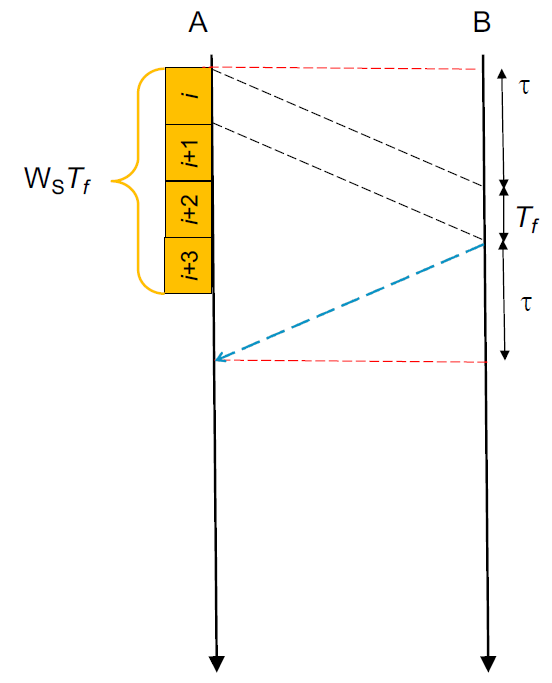
\includegraphics[scale=0.5]{selective_repeat_ack_out}
\end{center}
Dallo schema si evince che il tempo di trasmissione delle trame della finestra è pari a $W_ST_f$, mentre il primo ACK arriva non prima di $T_f+2\tau$ secondi, per cui la condizione per avere riscontri fuori dalla finestra di trasmissione è:
\begin{equation*}
    W_ST_f \leq T_f + 2\tau \Rightarrow W_S \leq 1 + 2a
\end{equation*}
Pertanto le espressione delle efficienze calcolate in precedenza vanno moltiplicate per un \textbf{fattore di perdita} che rappresenta il valore limite per GBN e SR nel caso di assenza di errori e riscontri fuori dalla finestra di trasmissione. Tale valore è dato dal rapporto tra tempo utile di occupazione del canale e tempo di attesa del primo riscontro:
\begin{equation*}
    \eta_W = \frac{W_ST_f}{T_f + 2\tau} = \frac{W_S}{1 + 2a}
\end{equation*}
Iniziamo applicando il fattore all'espressione dell'efficienza in SR:
\begin{equation*}
    \eta = (1 - P)\frac{W_S}{1 + 2a}
\end{equation*}
Per quanto riguarda il GBN è necessario fare un'altra considerazione. Si nota che nella sua espressione, K è proprio $W_S$ in quanto in caso di errore si ritrasmette l'intera finestra. Pertanto si ha:
\begin{equation*}
    \eta = \frac{(1 - P)}{1 + P(W_S - 1)}\frac{W_S}{1 + 2a}
\end{equation*}

\subsection{High Level Data Link Control Protocol}

\textbf{HLDC} è un protocollo datato, da cui ne sono derivati molti più moderni. Consiste nell'assegnare alle stazioni dei \textbf{ruoli}. In \textbf{configurazione sbilanciata} esiste un \textbf{master} (o primary) attraverso il quale tutti gli \textbf{slave} (o secondary) devono passare per inizializzare un collegamento o scambiare dati con un altro slave. Dunque questa configurazione è \textbf{half-duplex} (questa variante si chiama \textbf{Normal Response Mode}). Un'altra variante prende il nome di \textbf{Asynchronous Response Mode}, in cui le \textbf{stazioni slave trasmettono senza autorizzazione del master} ma sono comunque \textbf{supervisionate dal master} in maniera asincrona. Si può avere anche una \textbf{configurazione Peer-to-Peer}, detta \textbf{bilanciata}, tra due stazioni, ottenendo la possibilità di comunicare in modalità \textbf{full-duplex}. La struttura del frame è la seguente:
\begin{center}
    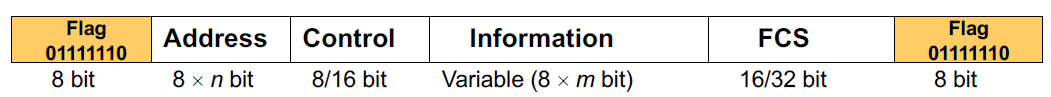
\includegraphics[scale=0.35]{hldc_frame}
\end{center}
Le flag non sono propriamente parte del frame, ma vengono aggiunte al passaggio a livello 1 (fisico) per delimitare dove inizia e dove termina un frame. I restanti campi sono:
\begin{itemize}
    \item \textbf{ADDRESS}: Indirizzo
    \begin{itemize}
        \item Del trasmettitore (se secondary)
        \item Del ricevitore (se primary)
        \item Tutti 1 (segnala trasmissione \textbf{broadcast})
    \end{itemize}
    \item \textbf{CONTROL}: Tipo di frame, numerazione e riscontro
    \item \textbf{INFORMATION}: Payload contenente i dati dal livello superiore
    \item \textbf{FCS}: Frame Check Sequence (\textbf{CRC} a 16 o 32 bit)
\end{itemize}

\subsection{Bit Stuffing}

Nel protocollo HLDC sorge un problema abbastanza evidente: potrebbe capitare che nel frame, \textbf{prima della sua effettiva conclusione}, vi sia una \textbf{sequenza di bit uguale alla flag} (01111110) che viene usata per delimitare inizio e fine frame. Per risolvere il problema bisogna modificare i bit in maniera tale da non avere più questa sequenza "incriminata", dando comunque la possibilità al ricevente di rimuovere i bit aggiunti e ottenere le informazioni originali. Nel Bit Stuffing si \textbf{inserisce uno 0 ogni cinque 1 ripetuti}. In ricezione, il ricevente sa già che questa procedura è stata applicata, quindi \textbf{rimuove lo 0 dopo cinque 1 ripetuti}. Lo svantaggio di questo metodo è che \textbf{si perde la molteplicità 8} dei dati, che in alcune situazioni è determinante. Ovviamente \textbf{le flag reali non vengono toccate da questa procedura}.

\subsection{Cyclic Redundancy Check}

Il valore calcolato mediante \textbf{algoritmo CRC} (a 16 o 32 bit) viene inserito nel campo \textbf{FCS} del frame. Il CRC è \textbf{molto efficiente} perché può essere implementato sfruttando dei semplici circuiti elettronici. Per funzionare sfrutta l'algebra dei campi finiti (di Galois). I passaggi dell'algoritmo sono i seguenti:
\begin{itemize}
    \item Viene definito un \textbf{polinomio G(x)} detto \textbf{GENERATORE}, \textbf{fisso e noto sia al mittente che al destinatario}. In genere viene \textbf{stabilito dal protocollo}. È un polinomio di grado r (quindi ha r + 1 coefficienti), ed è rappresentabile in binario: ad esempio $G(x) = x^3 + x^2 + 1$ diventa la sequenza 1101 (infatti in questo caso r = 3). Dunque il valore di r deve essere necessariamente pari al numero di bit in FCS;
    \item A partire dai d bit del payload + header, si crea un polinomio P(x) di grado d - 1;
    \item Si moltiplica P(x) per $x^r$ ottenendo il polinomio $x^rP(x)$ di grado d + r - 1 (ha d + r coefficienti). Questo logicamente equivale a uno shift a sinistra di r posti dei bit di P(x);
    \item Si ottiene quindi un FCS di tutti 0 (perché la lunghezza del FCS è di r bit);
    \item Si divide $x^rP(x)$ per G(x) effettuando la divisione aritmetica modulo 2 (si usa l'operatore \textbf{XOR} invece della somma):
    \begin{equation*}
        \frac{x^rP(x)}{G(x)} = Q(x) \oplus \frac{R(x)}{G(x)}
    \end{equation*}
    Si nota che \textbf{R(x) avrà grado al più r - 1} (r coefficienti);
    \item \textbf{I bit di R(x) costituiscono i bit del CRC} che vengono posti nel campo FCS. Per inserirli effettuo una XOR tra i bit di $x^rP(x)$ e di R(x). La trama finale trasmessa sarà rappresentabile con il polinomio $P^{Tx}(x)$, di grado d + r - 1:
    \begin{equation*}
        P^{Tx}(x) = x^rP(x) \oplus R(x)
    \end{equation*}
\end{itemize}
In ricezione, il destinatario sfrutta la \textbf{condizione necessaria del CRC} per verificare l'esattezza della trama. La condizione necessaria affinché non ci sia errore (CRC corretto) è che \textbf{sia nullo il resto della divisione tra il polinomio creato dalla trama ricevuta e il polinomio generatore}, ossia data la divisione:
\begin{equation*}
    \frac{P^{Rx}(x)}{G(x)} = Q'(x) \oplus R'(x)
\end{equation*}
Deve essere $R'(x) = 0$. Questa \textbf{condizione è necessaria ma non sufficiente a garantire che l'errore non ci sia}. Esiste infatti sempre una probabilità non nulla di avere il famoso \textbf{errore di sistema}. Comunque \textbf{in caso di errore ($R'(x) \neq 0$) si ha l'assoluta certezza dell'errore}, il che è una gran cosa.

\subsubsection{Dimostrazione della condizione necessaria}

In assenza di errori, la trama ricevuta è necessariamente uguale a quella trasmessa, quindi si ha:
\begin{equation*}
    P^{Rx}(x) = P^{Tx}(x)
\end{equation*}
Dividendo tutto per G(x), si ha che:
\begin{equation*}
    \frac{P^{Rx}(x)}{G(x)} = \frac{P^{Tx}(x)}{G(x)} = \frac{x^rP(x) \oplus R(x)}{G(x)} = \frac{x^rP(x)}{G(x)} \oplus \frac{R(x)}{G(x)}
\end{equation*}
La prima divisione è nota per come è stato costruito il CRC, per cui - ricordando che due bit uguali in XOR danno 0 e che un bit in XOR con 0 resta invariato - si ha la tesi:
\begin{equation*}
    \frac{x^rP(x)}{G(x)} \oplus \frac{R(x)}{G(x)} = Q(x) \oplus \frac{R(x)}{G(x)} \oplus \frac{R(x)}{G(x)} = Q(x)\ \blacksquare
\end{equation*}

\subsection{Point-to-Point Protocol}

L'obiettivo del PPP è stabilire come i pacchetti del livello superiore vengono incapsulati e inviati. È un \textbf{protocollo di livello 2}, definito dagli standard IETF RFC 1661, 1662. Il suo frame è il seguente:
\begin{center}
    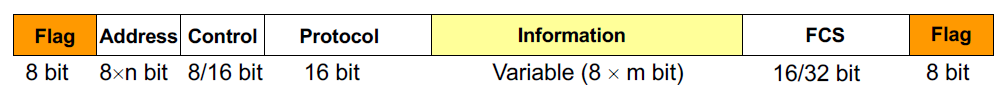
\includegraphics[scale=0.35]{ppp_frame}
\end{center}
\begin{itemize}
    \item \textbf{ADDRESS}: Sempre 11111111 (\textbf{broadcast})
    \item \textbf{CONTROL}: Sempre 00000011 (U frame)
    \item \textbf{INFORMATION}: Da 0 a 1500 byte
\end{itemize}
Il PPP lavora accoppiato ad altri due protocolli per gestire il collegamento:
\begin{itemize}
    \item \textbf{LCP (Link Control Protocol)}: Serve ad \textbf{aprire la connessione} e \textbf{negoziare i parametri} (compressione, criptazione, autenticazione PAP o CHAP, massima unità di ricezione). In autenticazione \textbf{PAP (Password Authentication Protocol)}, le credenziali (username e password) del mittente sono trasmessi in \textbf{cleartext}, e il ricevitore comunica se le ha accettate o rifiutate. In autenticazione \textbf{CHAP (Challenge HAndshake Protocol)} il destinatario invia una challenge al mittente da risolvere usando una \textbf{1-way hash function} (ad esempio MD5)
    \item \textbf{NCP (Network Control Protocol)}: Serve a scegliere e configurare uno o più protocolli di livello 3 (ad esempio IP)
\end{itemize}

\subsection{Byte Stuffing}

Anche il PPP usa la medesima flag di HLDC per delimitare inizio e fine del frame (01111110, 0x7E), ma \textbf{PPP non vuole rompere la molteplicità 8} delle informazioni (averla rende l'operazione di processing più efficiente), quindi effettua il \textbf{Byte Stuffing} invece del Bit Stuffing. In Byte Stuffing si \textbf{antepone un intero byte prima della sequenza "incriminata" 0x7E}. Il byte anteposto è \textbf{0x7D} (01111101). La sequenza 0x7E viene poi rimpiazzata dalla sequenza \textbf{0x5E} (1011110), che è ottenuta come \textbf{XOR tra 0x7D e 0x20} (0010000). Quando il ricevitore vede il byte 0x7D, sa che il byte successivo andrà messo in XOR con 0x20 per riottenere i byte originali. \textbf{Questo stesso procedimento è applicato sulla stessa sequenza 0x7D} (viene trasmesso 0x7D, 0x5D) \textbf{per evitare inconsistenze} (se non ci fosse questa protezione il ricevitore sbaglierebbe i byte perché senza sapere niente farebbe lo XOR di 0x20 con il byte che sta dopo 0x7D, come è solito fare). Inoltre è anche applicato sulla sequenza di control (0x03, viene trasmesso 0x7D, 0x23).

\subsection{Protocollo ALOHA}

È un \textbf{protocollo di accesso multiplo casuale senza rilevazione del canale} (detto facile, le stazioni trasmettono quando vogliono e non controllano nulla). Vi è un \textbf{ACK} quando il ricevente segnala la corretta ricezione, che arriva solitamente su un canale a parte. \textbf{In caso di collisione, l'ACK non arriva} e il mittente considera persa la trama dopo $2\tau$. Non conviene ritrasmettere subito la trama perché il canale potrebbe essere ancora occupato. Si aspetta un tempo casuale (detto \textbf{Backoff Time}), valorizzato estraendo un \textbf{numero casuale} i compreso\textbf{ tra 0 e K} (K$\geq$2 costante stabilita a priori) e \textbf{moltiplicandolo per T} (tempo di trasmissione della trama). Vi è una piccola probabilità che due stazioni estraggano lo stesso numero, in tal caso ci sarà sicuramente una collisione e il processo è ripetuto.

\subsubsection{Throughput in ALOHA}

Sia $\Lambda_s$ il \textbf{numero medio di pacchetti emesso} dalla sorgente, $\Pi$ la \textbf{probabilità che il pacchetto non arrivi o arrivi errato} (viene scartato).
Si ipotizza che la \textbf{probabilità di collisione degli ACK} sia \textbf{trascurabile}, che siano presenti \textbf{infinite stazioni, ciascuna che genera traffico infinitesimo}. \textbf{Ogni stazione trasmette indipendentemente dalle altre}. In queste ipotesi abbastanza stringenti, le stazioni si comportano secondo un \textbf{processo di Poisson}. Per i calcoli è necessario introdurre il concetto di \textbf{tempo di vulnerabilità}: intervallo di tempo durante il quale se due o più stazioni tentano di trasmettere, si avrà sicuramente una collisione. Questo tempo \textbf{in ALOHA è pari a 2T}, perché oltre al tempo di T del pacchetto corrente c'è anche da considerare il T del pacchetto precedente.
\begin{center}
    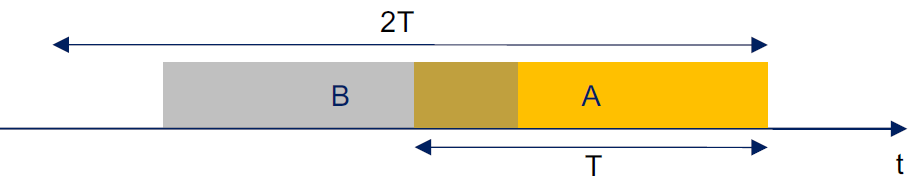
\includegraphics[scale=0.3]{aloha_vulnerability}
\end{center}
Per cui la probabilità $1 - \Pi$ è la probabilità di avere 0 pacchetti trasmessi in 2T, cioè la probabilità di avere 0 eventi nel processo di Poisson:
\begin{equation*}
    p_k = \frac{(\lambda t)^k}{k!}e^{-\lambda t} \Rightarrow p_0 = \frac{(\Lambda_s2T)^0}{0!}e^{-\Lambda_s2T} = e^{-\Lambda_s2T}
\end{equation*}
Pertanto il throughput sarà:
\begin{equation*}
    \Lambda_T = \Lambda_s(1 - \Pi) = \Lambda_s p_0 = \Lambda_se^{-\Lambda_s2T}\  \left[\frac{packet}{s}\right]
\end{equation*}
Per passare a bit/s basta moltiplicare per \textbf{L} (\textbf{lunghezza media dei pacchetti} misurata in bit/packet):
\begin{equation*}
    \Gamma_T = \Lambda_sLe^{-\Lambda_s2T}\ \left[\frac{bit}{s}\right]
\end{equation*}
Per normalizzare si divide per \textbf{C} (\textbf{frequenza di cifra} del canale):
\begin{equation*}
    S = \Lambda_s\frac{L}{C}e^{-\Lambda_s2T} = \Lambda_s T e^{-\Lambda_s2T} = Ge^{-2G}
\end{equation*}
Con \textbf{G} si indica il \textbf{traffico medio normalizzato} emesso dalla sorgente e \textbf{può essere anche maggiore di 1} (in tal caso si stanno mandando più bit di quanti lo stesso canale riesce a supportare, con perdita sicura della quota eccedente C). Studiando questa funzione (in variabile G) si ha che il throughput massimo normalizzato di ALOHA è ~0.18 per G = 0.5, ossia è del 18\% con traffico offerto pari al 50\% della capacità del canale.
\begin{center}
    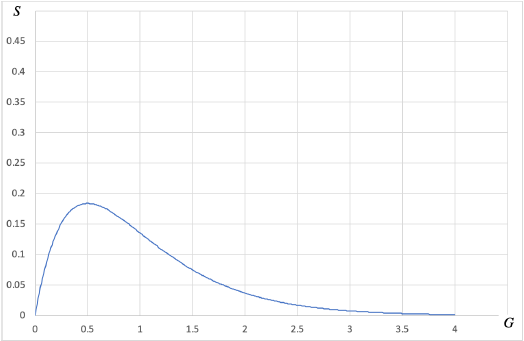
\includegraphics[scale=0.5]{aloha_throughput}
\end{center}

\subsubsection{Variante ALOHA Slotted e il suo throughput}

Se si ha a disposizione la \textbf{possibilità di sincronizzare tra loro tutte le stazioni} si può migliorare notevolmente il sistema, introducendo la \textbf{variante ALOHA Slotted}. Si \textbf{suddivide il tempo in slot di dimensione fissa pari a T}. \textbf{Quando una stazione vuole trasmettere, la si differisce al time slot successivo}. Le stazioni, essendo sincronizzate, presentano i medesimi slot temporali. Il risultato è che il \textbf{tempo di vulnerabilità si dimezza}: ora è T perché si avrà collisione solo se due stazioni trasmettono entro T e sono allocate allo stesso slot successivo.
\begin{center}
    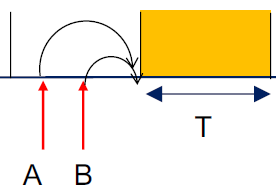
\includegraphics[scale=0.5]{aloha_slotted_collision}
\end{center}
Il modello per il calcolo del throughput è identico a quanto visto in ALOHA, ma la differenza sostanziale sta proprio nel tempo di vulnerabilità ora dimezzato, per cui i calcoli sono identici, ma dove c'era 2T ora c'è solo T:
\begin{equation*}
    p_0 = \frac{(\Lambda_sT)^0}{0!}e^{-\Lambda_sT} = e^{-\Lambda_sT}
\end{equation*}
\begin{equation*}
    \Lambda_T = \Lambda_s(1 - \Pi) = \Lambda_s p_0 = \Lambda_se^{-\Lambda_sT}\  \left[\frac{packet}{s}\right]
\end{equation*}
\begin{equation*}
    \Gamma_T = \Lambda_sLe^{-\Lambda_sT}\ \left[\frac{bit}{s}\right]
\end{equation*}
\begin{equation*}
    S = \Lambda_s\frac{L}{C}e^{-\Lambda_sT} = \Lambda_s T e^{-\Lambda_sT} = Ge^{-G}
\end{equation*}
Studiando questa funzione (in particolare la sua derivata prima), si ottiene $S_{MAX} \cong 0.37$, ossia un throughput massimo normalizzato del 37\% con G = 1 (ALOHA Slotted è in grado di sfruttare a pieno la capacità del canale). Un risultato decisamente migliore di ALOHA standard. Ovviamente, si nota che se G cresce troppo il throughput crolla, perché aumentano le stazioni che vogliono trasmettere (aumentando il traffico medio).

\subsection{Protocollo CSMA-CD}

Il \textbf{CSMA-CD} è un protocollo di tipo \textbf{CSMA (Carrier Sense Multiple Access)} in cui \textbf{è possibile individuare le collisioni mentre si inviano i primi bit e agire di conseguenza} (\textbf{Collision Detection}). Il funzionamento è semplice: se il canale è libero (Carrier Sense), la stazione inizia a trasmettere i primi bit della trama e mentre lo fa continua ad ascoltare il canale (si dice \textbf{Listening While Talking}). In questo modo è possibile accorgersi subito dell'eventuale collisione (causata da un altro flusso già attivo sul canale) \textbf{confrontando le sue onde elettromagnetiche con quelle del canale}. A collisione individuata, interrompe bruscamente la trasmissione ed emette un segnale detto \textbf{JAM}, che fa capire a tutte le altre stazioni connesse che c'è stata una collisione. Poiché nel canale condiviso tutti leggono i bit, tutti vengono a sapere della collisione e cancellano quei bit iniziali dai loro buffer di ricezione (comunque alla fine della trasmissione tutte le stazioni tranne il destinatario li avrebbero cancellati), e soprattutto rischedulano le proprie trasmissioni sulla base di un \textbf{algoritmo di backoff} (tecnica \textbf{no-persistent} in CSMA, algoritmo tipico usato è l'exponential backoff). Per realizzare tutto questo \textbf{è necessario che sia possibile a livello fisico una comunicazione di tipo full-duplex} (altrimenti non sarebbe possibile ascoltare mentre si inviano i dati). In alcuni canali (ad esempio il \textbf{canale radio}) non è possibile implementare il CSMA-CD perché le distanze rendono \textbf{inaffidabile la comparazione delle onde elettromagnetiche} (fondamentali affinché la CD funzioni).

\subsubsection{Lunghezza minima del frame}

Per garantire il corretto funzionamento di CSMA-CD i frame devono avere una lunghezza minima. Consideriamo il caso peggiore: nodi A e B più lontani possibile sul mezzo condiviso. B ascolta il canale un $\epsilon$ prima che gli arrivi il primo bit di A e invia i suoi primi bit, ma si accorge subito che il canale è occupato e manda il JAM. Il problema è che A non si accorge della collisione con B perché i bit gli arrivano dopo $\tau$ secondi, quindi per accorgersi della collisione si deve avere $T_f \geq 2\tau$, come in figura.
\begin{center}
    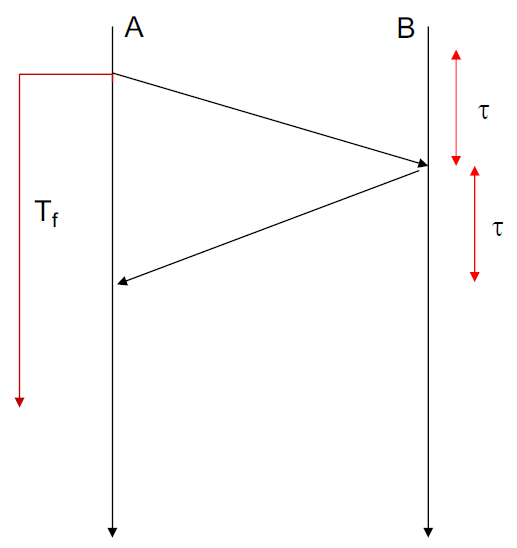
\includegraphics[scale=0.4]{csma_cd_frame_min_length}
\end{center}
Da cui si ricava che:
\begin{equation*}
    T_f = \frac{L_f}{C} \geq 2\tau = \frac{2d}{v} \Rightarrow L_f \geq \frac{2dC}{v}
\end{equation*}
La lunghezza minima del frame dipende dalla frequenza di cifra del canale C.

\subsection{Protocollo CSMA-CA}

Il protocollo \textbf{CSMA-CA} si realizza in canali in cui il mezzo condiviso non consente di individuare con abbastanza affidabilità le collisioni (ad esempio il \textbf{canale radio}). Il funzionamento è semplice: se il canale è libero (Carrier Sense), la stazione trasmette i frame mettendo nell'header un campo detto \textbf{DURATION}, che dichiara \textbf{per quanto tempo la stazione occuperà il canale} per la trasmissione del frame, considerando anche $\tau$ e $T_{ACK}$. Tutte le altre stazioni leggeranno quel campo e sapranno che in quell'intervallo di tempo il canale è occupato (quindi se tentassero di trasmettere ci sarebbe sicuramente collisione). Settano dunque al loro interno un timer detto \textbf{NAV (Network Allocation Vector)} e lo fanno partire. Finché NAV$>$0, le stazioni non effettuano il Carrier Sense (si dice che fanno "\textbf{virtual sensing}"). Allo scadere del NAV si ritenta l'ascolto del canale e se lo si sente libero si schedula la trasmissione.

\subsection{Problema del nodo nascosto}

Si manifesta nelle \textbf{WLAN}. Supponiamo di avere 3 nodi A, B e C posti in modo tale che B riesca a sentire e parlare con A e C, ma A e C non siano nel relativo range di copertura (essendo troppo distanti).
\begin{center}
    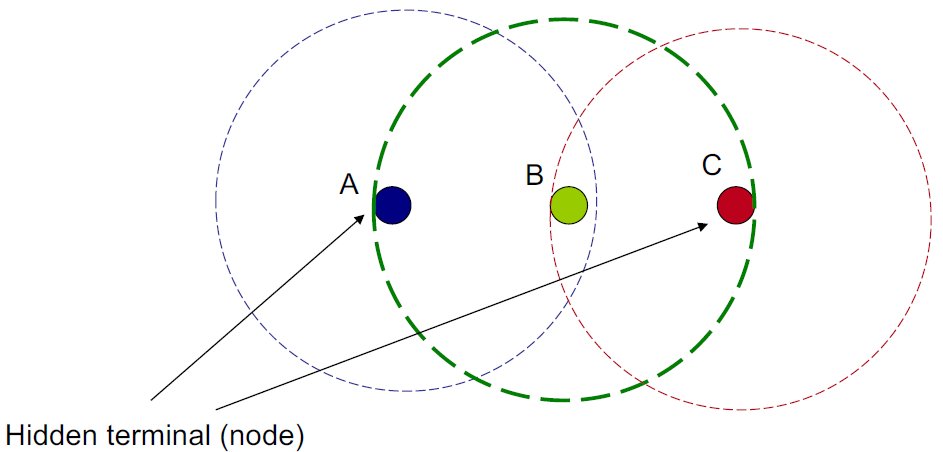
\includegraphics[scale=0.5]{hidden_terminal_problem}
\end{center}
Supponiamo ora che A e C vogliano parlare con B. A sentirà il canale libero (in WLAN si usa CSMA-CA) e inizierà a trasmettere a B. La stessa cosa accade per C. \textbf{Entrambi causeranno una collisione senza rendersene conto}. Per risolvere si usa la tecnica \textbf{RTS-CTS}: A e C, prima di trasmettere a B i loro dati, inviano un pacchetto molto piccolo detto \textbf{RTS} (\textbf{Request To Send}, 20 byte). Visto che RTS è piccolo la probabilità di collisione è molto bassa, quindi è verosimile che uno dei due RTS giunga prima a B. Nell'RTS è comunque presente il valore di DURATION per CSMA-CA. B vede il primo RTS che gli arriva, e risponde con un altro pacchetto piccolo detto \textbf{CTS} (\textbf{Clear To Send}, 14 byte) in cui comunicherà alla stazione cui RTS è arrivato prima che è possibile trasmettere. La stazione che non ha "vinto" la gara, riceve il CTS e leggendolo scopre di non aver "vinto" (non è possibile trasmettere), e dunque prende la sconfitta sportivamente astenendosi dal comunicare settando il suo NAV alla DURATION scritta nel CTS (ritrasmessa da B). Il problema è stato dunque pienamente risolto, introducendo però una piccola complicazione nel sistema.
\begin{center}
    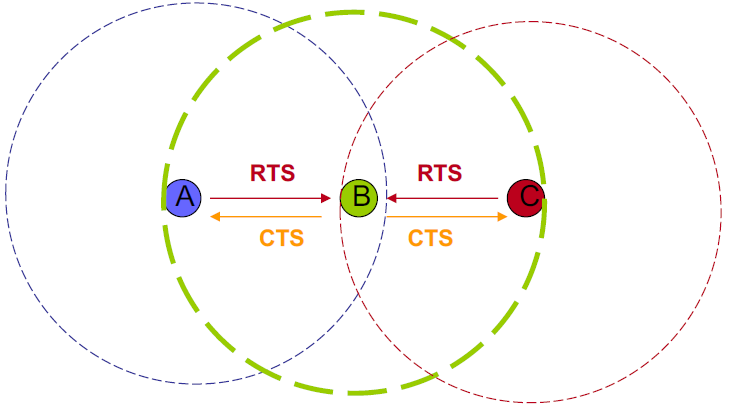
\includegraphics[scale=0.4]{hidden_terminal_problem_solution}
\end{center}

\subsection{Problema del nodo esposto}

Si supponga una situazione con i nodi posti in questo modo: $A \rightleftarrows B\ C \dashrightarrow D$. A riesce a vedere solo B, B vede A e C, C vede B e D.
\begin{center}
    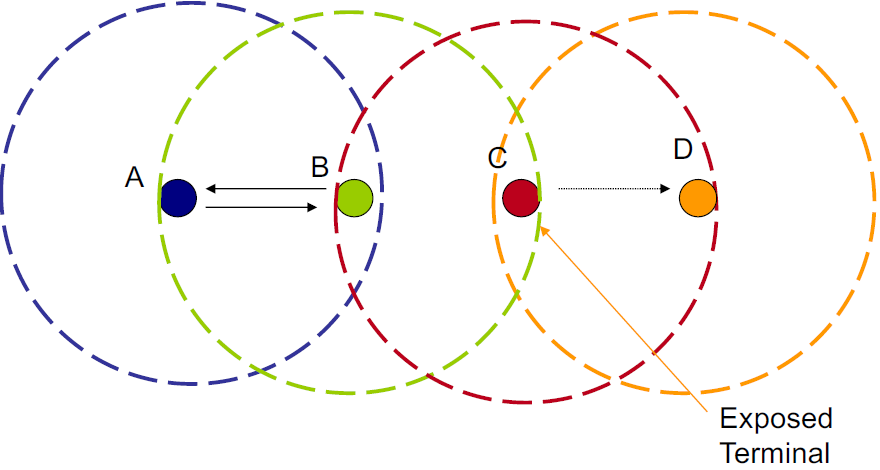
\includegraphics[scale=0.35]{exposed_terminal_problem}
\end{center}
Poiché A e B stanno parlando, fanno sempre contesa di canale con CSMA-CA. \textbf{C non riesce mai a parlare con D} perché non riesce mai a "vincere" la contesa con A e B (si dice che è "esposto"). Per risolvere il problema, si introduce il \textbf{BACKOFF ON SUCCESS}: quando un nodo invia correttamente una trama (viene riscontrata senza errori), avvia comunque un backoff time, in modo da dare ad altri nodi la possibilità di comunicare sul canale, riequilibrandone l'utilizzo medio da parte dei nodi. In questo modo C può comunicare con D e il problema è risolto.

\section{Domande sui bridge}

\subsection{Processo di bridging}

Il processo di bridging si divide in \textbf{due sotto-processi}: \textbf{FORWARDING} e \textbf{LEARNING}. È importante notare che i due sotto-processi accadono simultaneamente.
\begin{itemize}
    \item \textbf{FORWARDING} è il processo naturale, in cui il bridge/switch prende il pacchetto in ingresso e lo inoltra ad una particolare uscita.
    \item \textbf{LEARNING} è il processo in cui il bridge/switch "impara" e aggiorna la sua MAC Table sulla base del mittente del frame, perché quando gli arriva il frame capisce la porta a cui è collegato il MAC mittente e crea/aggiorna la sua relativa entry nella tabella.
\end{itemize}
Se, durante il FORWARDING, il dispositivo nota che la \textbf{porta} per raggiungere il destinatario \textbf{non è presente} (perché non è ancora stata acquisita dal sotto-processo LEARNING), \textbf{effettua un flooding} su tutte le porte eccetto quella in ingresso. Di seguito l'algoritmo dettagliato:
\begin{center}
    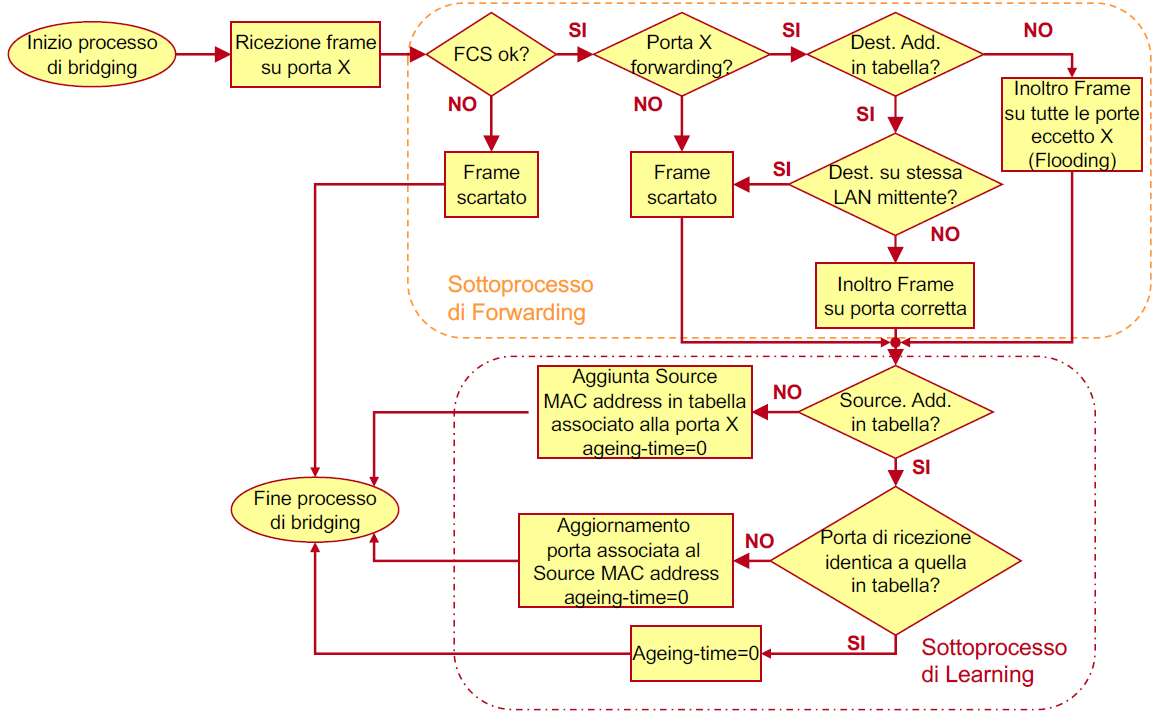
\includegraphics[scale=0.35]{bridging_process}
\end{center}

\subsection{Fasi dello Spanning Tree Protocol}

L'algoritmo \textbf{Spanning Tree} è definito dal protocollo IEEE 802.1d. Pone come obiettivo la risoluzione di un problema comune: può succede che i collegamenti fisici di un dispositivo di livello 2 siano collegati fra loro in modo da creare dei \textbf{loop} (a volte questi loop sono fatti volutamente ad arte per forzare strade alternative per alcuni flussi specifici). Il loop però è un problema serio a livello 2, perché \textbf{i dispositivi si scambiano pacchetti broadcast molto spesso} e quindi questi pacchetti \textbf{continueranno a ciclare} indefinitamente sulla rete (perché a livello 2 non c'è il campo TTL) fino a \textbf{saturare} l'intera banda, dunque bloccando l'intera rete. L'idea è di \textbf{disabilitare alcune porte} del dispositivo (operando sull'apposito campo \textbf{STATE} della \textbf{MAC Table} che di norma è sempre in stato "\textbf{forwarding}"), allo scopo di \textbf{creare un albero} che interconnetta tutti i dispositivi. L'albero è una struttura topologica naturalmente priva di loop, quindi il problema si risolve. L'algoritmo, quindi, gestisce dinamicamente le porte in modo tale da mantenere questa struttura ad albero ed evitare guasti. Le fasi principali dello Spanning Tree sono:
\begin{itemize}
    \item \textbf{Elezione del Root Bridge}: Viene scelto il bridge che farà da radice dell'albero
    \item \textbf{Selezione delle Root Port}: Vengono stabilite quali sono le porte dei bridge che si collegano a monte verso la root. Può accadere che in alcuni pezzi di LAN ci siano più bridge collegati ad una stessa porzione di LAN. In quel caso avviene un'ulteriore fase, ossia la:
    \item \textbf{Selezione della Designated Port}: Viene scelta le porta dei bridge (tra quelli collegati alla stessa porzione di LAN) che inoltrerà i frame. La porta scelta viene posta in forwarding state, le altre in blocking state.
\end{itemize}
Prima di proseguire con un'analisi delle fasi, è necessario introdurre il concetto di \textbf{Bridge Protocol Data Unit (BPDU)}. Le BPDU vengono usate al fine di realizzare le fasi dell'algoritmo. Periodicamente, tutti i bridge si scambiano questi frame (incapsulati dentro LLC e sempre inviati all'indirizzo multicast noto 01:80:C2:00:00:00). I bridge riconoscono questo indirizzo ed elaborano la BPDU (se lo Spanning Tree è stato abilitato nelle impostazioni del dispositivo). Esistono 2 tipi di BPDU:
\begin{itemize}
    \item \textbf{CONFIGURATION}: Usate per creare l'albero in prima configurazione iniziale.
    \item \textbf{TOPOLOGY CHANGE NOTIFICATION}: Usate per notificare un cambiamento topologico (causato da un guasto e/o spegnimento di uno o più bridge).
\end{itemize}

\subsubsection{Elezione del Root Bridge}

Alla prima configurazione o dopo il cambiamento topologico \textbf{ogni bridge si autodefinisce Root Bridge} e invia delle Configuration BPDU con \textbf{Root ID} pari al suo \textbf{Bridge ID} ogni \textbf{Hello Time} (di solito 2 secondi). Il Bridge ID è formato dall'unione di \textbf{Bridge Priority} e \textbf{Bridge MAC Address}. Se un bridge riceve una Configuration BPDU in cui il \textbf{Bridge ID è minore del proprio, lo riconosce come Root Bridge} e smette di mandare BPDU. Da quel momento inoltra solo quelle che riceve. Con questo processo si ha (dopo un intervallo di tempo abbastanza lungo) che il \textbf{Root Bridge sarà il bridge con identificativo più basso}. Se un bridge non riceve più BPDU per un periodo superiore al campo \textbf{Max Age}, viene nuovamente avviato il processo di elezione. È importante notare che \textbf{è possibile forzare il Root Bridge} che si vuole ottenere cambiando la priority in maniera tale da far sempre eleggere, ad esempio, un dispositivo più performante.
\begin{center}
    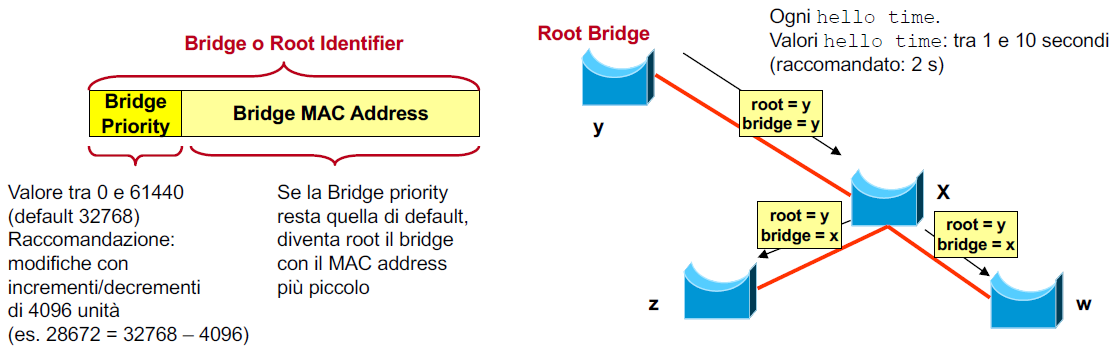
\includegraphics[scale=0.25]{spanning_tree_root_bridge}
\end{center}

\subsubsection{Selezione delle Root Port}

I bridge, prima di inoltrare le BPDU, aggiornano il \textbf{Path Cost}, pari in genere a 1000 diviso la velocità della rete in Mbps. Il Root Bridge genera sempre Path Cost = 0. Il Path Cost calcolato viene sommato a quello ricevuto. Se si ricevono più BPDU le si confronta, e diventa Root Port la porta che soddisfa, in ordine di importanza, queste condizioni: costo minimo, Bridge ID minimo, Port ID minimo, Port ID minimo tra i valori associati alle porte.
\begin{center}
    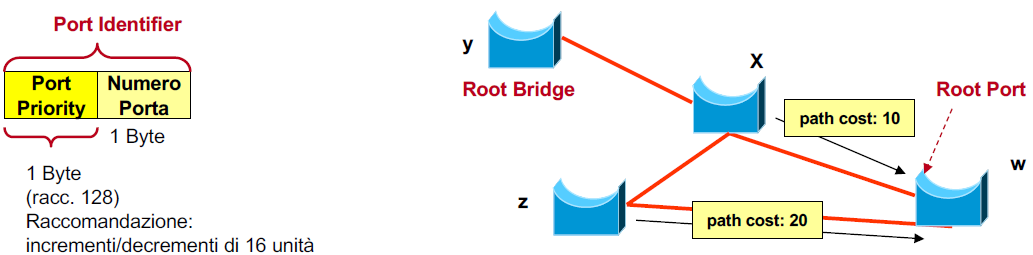
\includegraphics[scale=0.5]{spanning_tree_root_port}
\end{center}

\subsubsection{Selezione della Designated Port}

Quando si determina la Root Port, \textbf{tutte le porte tranne la Root Port passano in blocking state}. A questo punto, \textbf{se due bridge sono sulla stessa porzione di LAN}, ricevono BPDU da bridge che non sono root. Se una Configuration BPDU è ricevuta da una di queste porte a \textbf{priorità più bassa}, quest'ultima diventa la Designated Port, e pongo quelle a \textbf{maggiore priorità in blocking state}.
\begin{center}
    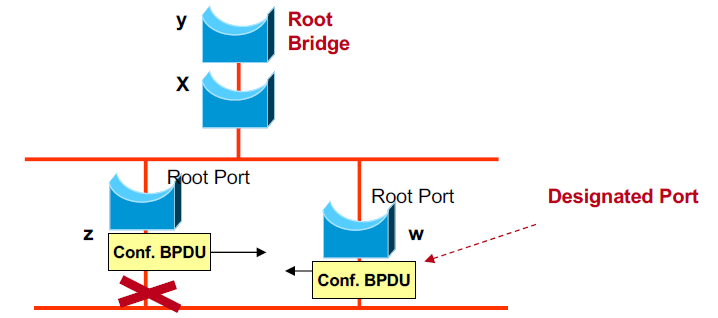
\includegraphics[scale=0.5]{spanning_tree_designated_port}
\end{center}

\end{document}
